\chapter{Simulation}
All components for the subsystems have now been designed, which leads to a simulation of the full system to make sure the system will be performing as expected when implemented in the DSP. The full system has 7 downsampling stages, which mean that the Fs will be $Fs/128=375 Hz$.The decimation filter has a delay of 25 samples  while the interpolation filter has a delay of 17 samples, therefore the band after the different downsampling stages must be delayed correctly so the bands can be summed up in phase. 

To calculate the delays the following formula is used for every band:
\begin{equation}
Z^{-d}_{band} = (M_{Int}/2) + \sum_{n=1}^{6} ((M_{Dec}/2)\cdot 2^n+(M_{Int}/2)\cdot 2^n) = 5309\enhed{samples}
\label{eq:delays}
\end{equation}
Band 2: 2621 sample delay (n going from 1 to 5). \\
Band 3: 1277 sample delay (n going from 1 to 4). \\
Band 4: 605 sample delay (n going from 1 to 3). \\
Band 5: 269 sample delay (n going from 1 to 2). \\
Band 6: 101 sample delay (n going from 1 to 1). 

While the last delay in band 8 is only the delay of the interpolation filter which equals 17: \\
Band 7: 17 sample delay.


On \autoref{fig:OverallSimulation} an outline of the entire system is depicted. It shows how a signal is applied to the first downsampling and then applied to the following consecutive downsamplings. When the signal has reached the four lowest band, a RMS compressor is applied. Each band is delayed according to the calculated delays, upsampled and summed together, whiched is outputted.

\begin{figure}[H]
\centering
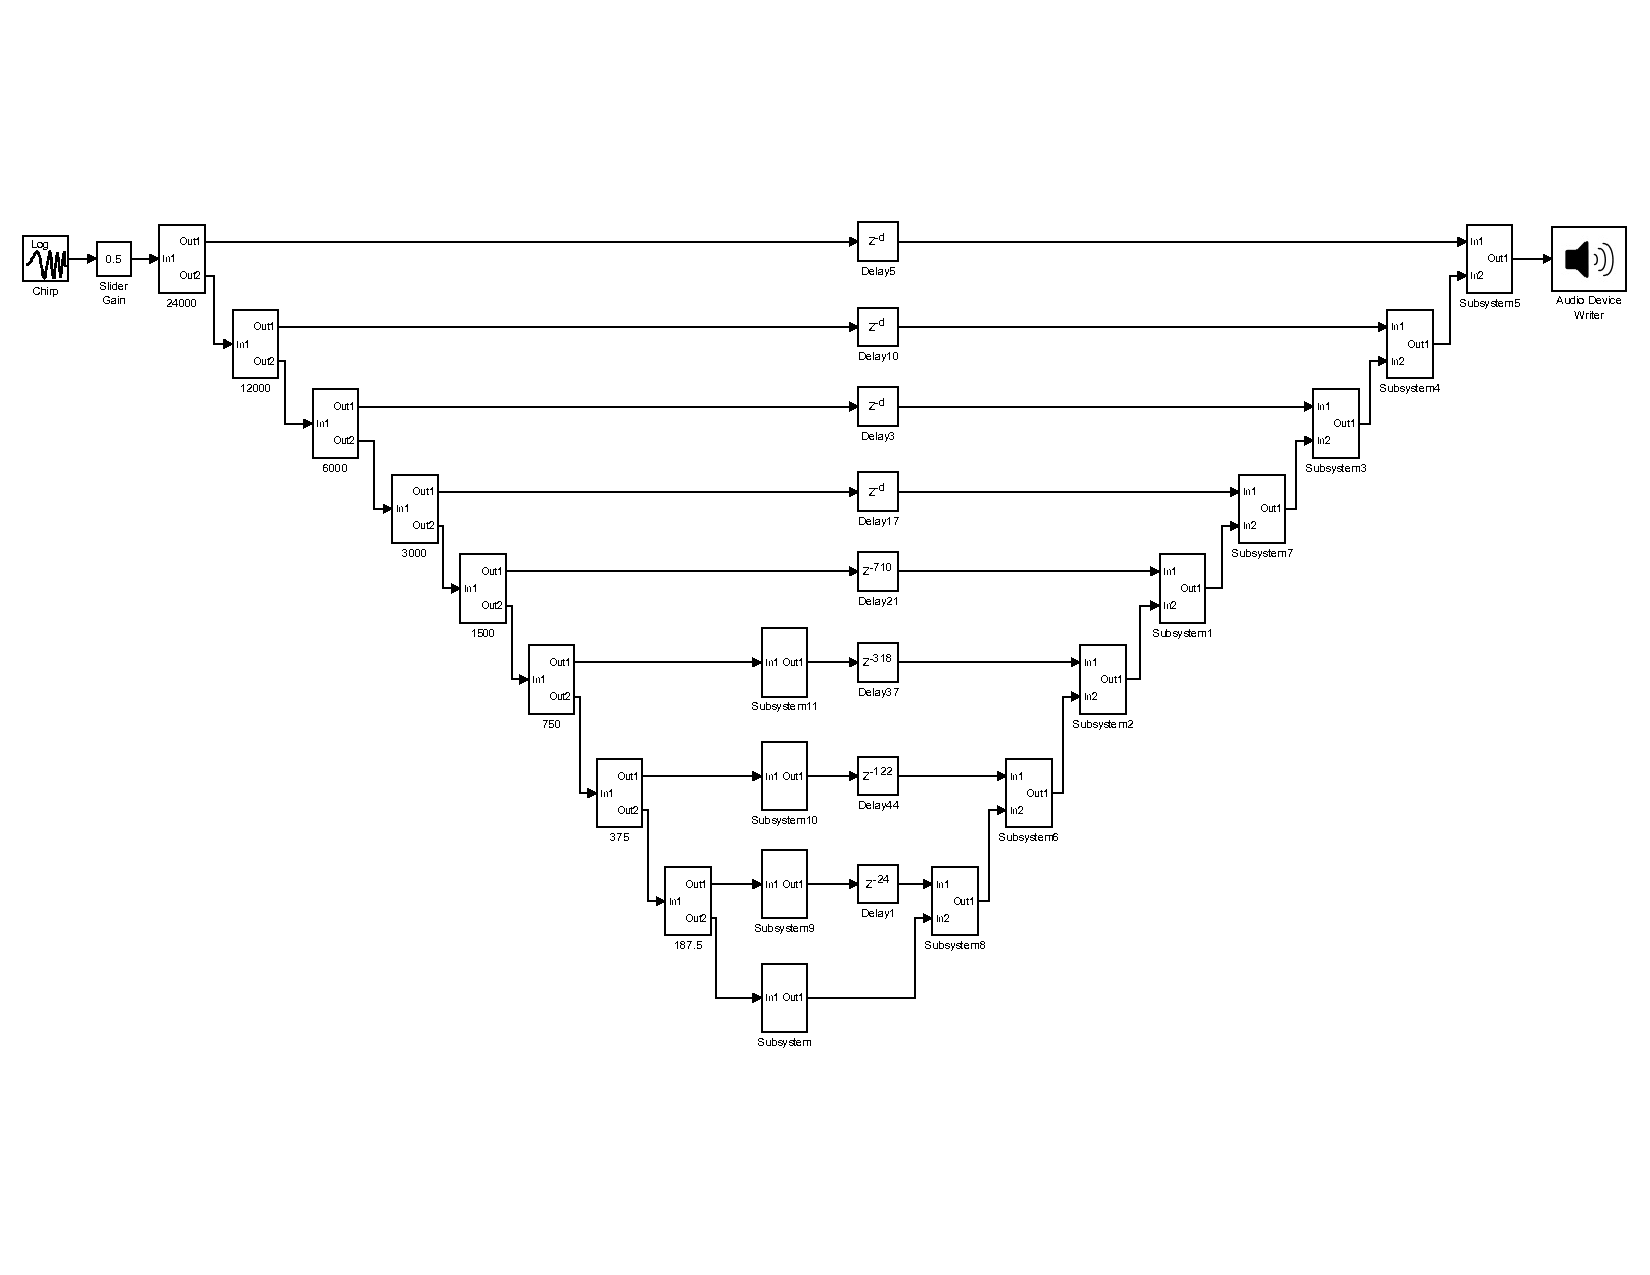
\includegraphics[width=\textwidth,angle=90, page=1]{Simulation}
\label{fig:OverallSimulation}
\caption{Overall view of the system used for simulation in Simulink.}
\end{figure}

In the simulation the following subsystem depicted on \autoref{fig:SubsystemSimulation}, are used. On \autoref{fig:DownsamplingSimulation} the downsampling system is shown. It shows how the signal is first filtered followed by subtracting it from the original signal and finally downsampled. \autoref{fig:UpsamplingSimulation} shows the upsampling system where it shows how the upsampling flow of the signal is. Namely how the signal is zero-padded followed by an lowpass filtering and then applied a gain of 2 corresponding with the up-samplings factor. \autoref{fig:RMSCompressorSimulation} Shows the compressor algorithm applied in the simulation. The compressor calculates the RMS where an if statement determined whether a gain of 1 or the model should be used. When the gain has been determined it is multiplied on before being ready for up-sampling. 
\begin{figure}[H]
\centering
\begin{subfigure}[t]{0.49\textwidth}
    \centering
\includegraphics[width=\textwidth, page=2]{Simulation}
    \caption{Decimaation subsystem.}
    \label{fig:DownsamplingSimulation}
\end{subfigure}
\begin{subfigure}[t]{0.49\textwidth}
    \centering
\includegraphics[width=\textwidth, page=11]{Simulation}
    \caption{Interpolation subsystem.}
    \label{fig:UpsamplingSimulation}
\end{subfigure}
\begin{subfigure}[t]{\textwidth}
    \centering
\includegraphics[width=\textwidth, page=13]{Simulation}
    \caption{RMS Compressor subsystem.}
    \label{fig:RMSCompressorSimulation}
\end{subfigure}
\label{fig:SubsystemSimulation}
\caption{View of the subsystems found in figure \ref{fig:OverallSimulation}}
\end{figure}


During the simulation the following settings has been applied to the subsystems:
\begin{itemize}
\item The filters, both up and down-sampling has been fitted with quantized filter coefficients corresponding with a 16-bit fixed point architecture.
\item The RMS compressor is fitted with a threshold of 0.2 
\item The up and down-samplings factor is 2.
\end{itemize}

\section{10 second simulation}
Under the simulation, the following settings are set/applied:
\begin{itemize}
\item The sampling frequency is 48 kHz.
\item The test signal played with an amplitude of 0.5.
\item The test signal is a logarithmic sweep from 0 Hz to 500 Hz during a 10 second period.
\end{itemize}

The simulation file and needed scripts are found at \path{CD://something }



In the following section a 10 second simulation is showed with a graphical output of each band, showed in \autoref{fig:SimulationComparisson}. As described above, the signal is a sweep from 0 Hz to 500 Hz in a 10 seconds duration. On the graphs the following color codes are used:
\begin{itemize}
\item Blue shows the gain applied in each band
\item Red shows the RMS value calculated in the band
\item Black shows the output which is feed to the up-sampling system.
\end{itemize}

\begin{figure}[H]
\centering
\begin{subfigure}[t]{0.49\textwidth}
    \centering
    \tikzsetnextfilename{Band1Simulation}
    % This file was created by matlab2tikz.
%
%The latest updates can be retrieved from
%  http://www.mathworks.com/matlabcentral/fileexchange/22022-matlab2tikz-matlab2tikz
%where you can also make suggestions and rate matlab2tikz.
%
\definecolor{mycolor1}{rgb}{0.00000,0.44700,0.74100}%
\definecolor{mycolor2}{rgb}{0.85000,0.32500,0.09800}%
\definecolor{mycolor3}{rgb}{0.00,0.00,0.00}%
%
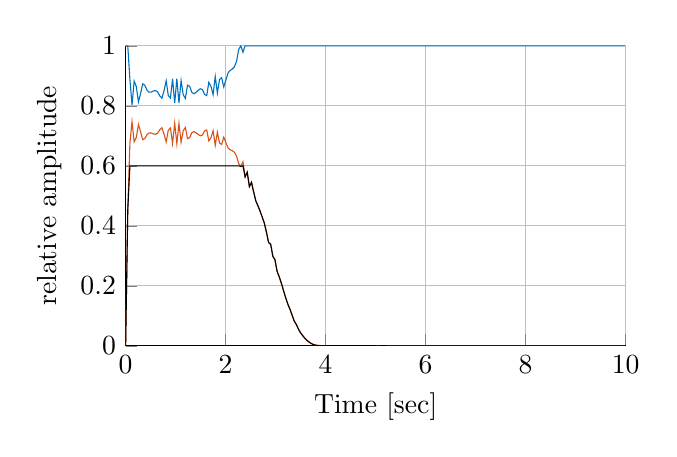
\begin{tikzpicture}

\begin{axis}[%
width=2.5in,
height=1.5in,
at={(0.758in,0.481in)},
scale only axis,
xmin=0,
xmax=10,
xlabel={Time [sec]},
xmajorgrids,
ymin=0,
ymax=1,
ylabel={relative amplitude},
ymajorgrids,
axis background/.style={fill=white},
axis x line*=bottom,
axis y line*=left
]
\addplot [color=mycolor1,solid,forget plot]
  table[row sep=crcr]{%
0	1\\
0.0426666666666667	1\\
0.0853333333333333	0.888215243570243\\
0.128	0.803091361874838\\
0.170666666666667	0.882454481383015\\
0.213333333333333	0.864255420335044\\
0.256	0.81341937565934\\
0.298666666666667	0.840737612391603\\
0.341333333333333	0.873414173309961\\
0.384	0.868181396512917\\
0.426666666666667	0.852430982426081\\
0.469333333333333	0.84535973003027\\
0.512	0.845988803510365\\
0.554666666666667	0.849304136659777\\
0.597333333333333	0.850966287890872\\
0.64	0.846137461214332\\
0.682666666666667	0.833053934284735\\
0.725333333333333	0.825514465304777\\
0.768	0.850322820099459\\
0.810666666666667	0.88331008362951\\
0.853333333333333	0.834143729974713\\
0.896	0.826054815883682\\
0.938666666666667	0.890043039790512\\
0.981333333333333	0.808737777633939\\
1.024	0.890775962342523\\
1.06666666666667	0.80931843021796\\
1.10933333333333	0.883995615033962\\
1.152	0.836560283216474\\
1.19466666666667	0.824600174516519\\
1.23733333333333	0.868738973552502\\
1.28	0.865108049319979\\
1.32266666666667	0.845205068138794\\
1.36533333333333	0.840283900418395\\
1.408	0.844785457081578\\
1.45066666666667	0.851493192568422\\
1.49333333333333	0.856933430712296\\
1.536	0.854210371997499\\
1.57866666666667	0.837731492715724\\
1.62133333333333	0.834028284329381\\
1.664	0.878295135603366\\
1.70666666666667	0.864985496704436\\
1.74933333333333	0.83705894619206\\
1.792	0.897702135634999\\
1.83466666666667	0.842350186893\\
1.87733333333333	0.887632946984465\\
1.92	0.893848685597325\\
1.96266666666667	0.862990480819975\\
2.00533333333333	0.885935457454018\\
2.048	0.909693580288854\\
2.09066666666667	0.918114143137892\\
2.13333333333333	0.92274784972839\\
2.176	0.930107502530443\\
2.21866666666667	0.948809166508671\\
2.26133333333333	0.988238797709705\\
2.304	1\\
2.34666666666667	0.978289579368019\\
2.38933333333333	1\\
2.432	1\\
2.47466666666667	1\\
2.51733333333333	1\\
2.56	1\\
2.60266666666667	1\\
2.64533333333333	1\\
2.688	1\\
2.73066666666667	1\\
2.77333333333333	1\\
2.816	1\\
2.85866666666667	1\\
2.90133333333333	1\\
2.944	1\\
2.98666666666667	1\\
3.02933333333333	1\\
3.072	1\\
3.11466666666667	1\\
3.15733333333333	1\\
3.2	1\\
3.24266666666667	1\\
3.28533333333333	1\\
3.328	1\\
3.37066666666667	1\\
3.41333333333333	1\\
3.456	1\\
3.49866666666667	1\\
3.54133333333333	1\\
3.584	1\\
3.62666666666667	1\\
3.66933333333333	1\\
3.712	1\\
3.75466666666667	1\\
3.79733333333333	1\\
3.84	1\\
3.88266666666667	1\\
3.92533333333333	1\\
3.968	1\\
4.01066666666667	1\\
4.05333333333333	1\\
4.096	1\\
4.13866666666667	1\\
4.18133333333333	1\\
4.224	1\\
4.26666666666667	1\\
4.30933333333333	1\\
4.352	1\\
4.39466666666667	1\\
4.43733333333333	1\\
4.48	1\\
4.52266666666667	1\\
4.56533333333333	1\\
4.608	1\\
4.65066666666667	1\\
4.69333333333333	1\\
4.736	1\\
4.77866666666667	1\\
4.82133333333333	1\\
4.864	1\\
4.90666666666667	1\\
4.94933333333333	1\\
4.992	1\\
5.03466666666667	1\\
5.07733333333333	1\\
5.12	1\\
5.16266666666667	1\\
5.20533333333333	1\\
5.248	1\\
5.29066666666667	1\\
5.33333333333333	1\\
5.376	1\\
5.41866666666667	1\\
5.46133333333333	1\\
5.504	1\\
5.54666666666667	1\\
5.58933333333333	1\\
5.632	1\\
5.67466666666667	1\\
5.71733333333333	1\\
5.76	1\\
5.80266666666667	1\\
5.84533333333333	1\\
5.888	1\\
5.93066666666667	1\\
5.97333333333333	1\\
6.016	1\\
6.05866666666667	1\\
6.10133333333333	1\\
6.144	1\\
6.18666666666667	1\\
6.22933333333333	1\\
6.272	1\\
6.31466666666667	1\\
6.35733333333333	1\\
6.4	1\\
6.44266666666667	1\\
6.48533333333333	1\\
6.528	1\\
6.57066666666667	1\\
6.61333333333333	1\\
6.656	1\\
6.69866666666667	1\\
6.74133333333333	1\\
6.784	1\\
6.82666666666667	1\\
6.86933333333333	1\\
6.912	1\\
6.95466666666667	1\\
6.99733333333333	1\\
7.04	1\\
7.08266666666667	1\\
7.12533333333333	1\\
7.168	1\\
7.21066666666667	1\\
7.25333333333333	1\\
7.296	1\\
7.33866666666667	1\\
7.38133333333333	1\\
7.424	1\\
7.46666666666667	1\\
7.50933333333333	1\\
7.552	1\\
7.59466666666667	1\\
7.63733333333333	1\\
7.68	1\\
7.72266666666667	1\\
7.76533333333333	1\\
7.808	1\\
7.85066666666667	1\\
7.89333333333333	1\\
7.936	1\\
7.97866666666667	1\\
8.02133333333333	1\\
8.064	1\\
8.10666666666667	1\\
8.14933333333333	1\\
8.192	1\\
8.23466666666667	1\\
8.27733333333333	1\\
8.32	1\\
8.36266666666667	1\\
8.40533333333333	1\\
8.448	1\\
8.49066666666667	1\\
8.53333333333333	1\\
8.576	1\\
8.61866666666667	1\\
8.66133333333333	1\\
8.704	1\\
8.74666666666667	1\\
8.78933333333333	1\\
8.832	1\\
8.87466666666667	1\\
8.91733333333333	1\\
8.96	1\\
9.00266666666667	1\\
9.04533333333333	1\\
9.088	1\\
9.13066666666667	1\\
9.17333333333333	1\\
9.216	1\\
9.25866666666667	1\\
9.30133333333333	1\\
9.344	1\\
9.38666666666667	1\\
9.42933333333333	1\\
9.472	1\\
9.51466666666667	1\\
9.55733333333333	1\\
9.6	1\\
9.64266666666667	1\\
9.68533333333333	1\\
9.728	1\\
9.77066666666667	1\\
9.81333333333333	1\\
9.856	1\\
9.89866666666667	1\\
9.94133333333333	1\\
9.984	1\\
};
\addplot [color=mycolor2,solid,forget plot]
  table[row sep=crcr]{%
0	0.000671601058471403\\
0.0426666666666667	0.453028783946894\\
0.0853333333333333	0.675511937386099\\
0.128	0.74711300417836\\
0.170666666666667	0.679921755351798\\
0.213333333333333	0.69423920970886\\
0.256	0.737626884672686\\
0.298666666666667	0.713659043150468\\
0.341333333333333	0.686959312471644\\
0.384	0.691099812101391\\
0.426666666666667	0.703869301292119\\
0.469333333333333	0.709757016670898\\
0.512	0.709229244536507\\
0.554666666666667	0.706460706007787\\
0.597333333333333	0.705080810530233\\
0.64	0.709104640206937\\
0.682666666666667	0.720241481741712\\
0.725333333333333	0.726819486777233\\
0.768	0.705614368822679\\
0.810666666666667	0.679263161510177\\
0.853333333333333	0.71930049755117\\
0.896	0.726344049405659\\
0.938666666666667	0.674124703161794\\
0.981333333333333	0.741896838002761\\
1.024	0.673570039342044\\
1.06666666666667	0.741364557629575\\
1.10933333333333	0.678736398457077\\
1.152	0.717222670066373\\
1.19466666666667	0.727625361408386\\
1.23733333333333	0.690656248040124\\
1.28	0.693554984804074\\
1.32266666666667	0.709886893273423\\
1.36533333333333	0.714044383929345\\
1.408	0.710239499236621\\
1.45066666666667	0.704644505953331\\
1.49333333333333	0.700171073383461\\
1.536	0.702403084379496\\
1.57866666666667	0.716219940657769\\
1.62133333333333	0.719400062651884\\
1.664	0.683141663522724\\
1.70666666666667	0.69365324885328\\
1.74933333333333	0.716795397420353\\
1.792	0.6683731453703\\
1.83466666666667	0.712292831812734\\
1.87733333333333	0.675955080349784\\
1.92	0.671254553111574\\
1.96266666666667	0.695256799854741\\
2.00533333333333	0.677250238662156\\
2.048	0.659562750579687\\
2.09066666666667	0.653513514070642\\
2.13333333333333	0.650231805120553\\
2.176	0.64508672209142\\
2.21866666666667	0.632371630859994\\
2.26133333333333	0.607140704646014\\
2.304	0.598056188892334\\
2.34666666666667	0.613315333878547\\
2.38933333333333	0.563244416925541\\
2.432	0.578515201450806\\
2.47466666666667	0.530850621279024\\
2.51733333333333	0.544626551361463\\
2.56	0.51304379472764\\
2.60266666666667	0.483407114390941\\
2.64533333333333	0.466930224187969\\
2.688	0.449233044304943\\
2.73066666666667	0.429683304968031\\
2.77333333333333	0.409072264258996\\
2.816	0.379077521453027\\
2.85866666666667	0.344508723126061\\
2.90133333333333	0.338148823116303\\
2.944	0.29829991436997\\
2.98666666666667	0.286862918840593\\
3.02933333333333	0.248165949059831\\
3.072	0.229980126789434\\
3.11466666666667	0.208979836545078\\
3.15733333333333	0.184177307536999\\
3.2	0.160486607450433\\
3.24266666666667	0.139531671956084\\
3.28533333333333	0.122595319879048\\
3.328	0.102888729286201\\
3.37066666666667	0.0828208655021142\\
3.41333333333333	0.0714126907783905\\
3.456	0.0555997742952173\\
3.49866666666667	0.0432452893503304\\
3.54133333333333	0.0339041905306332\\
3.584	0.0252206300108411\\
3.62666666666667	0.0179914806527692\\
3.66933333333333	0.0123291488734702\\
3.712	0.00771690793780233\\
3.75466666666667	0.00426970970393281\\
3.79733333333333	0.00229613061149498\\
3.84	0.000990451236761237\\
3.88266666666667	0.000808869747619119\\
3.92533333333333	0.00085629017863418\\
3.968	0.000780112929133348\\
4.01066666666667	0.000543513763057712\\
4.05333333333333	0.00023552450284778\\
4.096	0.000136837807567839\\
4.13866666666667	0.000353294555850783\\
4.18133333333333	0.00048503509759329\\
4.224	0.000510911293689333\\
4.26666666666667	0.000463621434241083\\
4.30933333333333	0.000340833946027341\\
4.352	0.00017515021497186\\
4.39466666666667	5.46416076322823e-05\\
4.43733333333333	0.000176963343337181\\
4.48	0.000266240379999868\\
4.52266666666667	0.0003244186746928\\
4.56533333333333	0.000312141942023658\\
4.608	0.00024872583958487\\
4.65066666666667	0.000160785529246407\\
4.69333333333333	6.13640346812659e-05\\
4.736	6.08096137174145e-05\\
4.77866666666667	0.000128386355010368\\
4.82133333333333	0.000174059611267489\\
4.864	0.000178777904249968\\
4.90666666666667	0.000156736569276186\\
4.94933333333333	0.000115227409006594\\
4.992	5.52350717469468e-05\\
5.03466666666667	2.01889797396134e-05\\
5.07733333333333	3.4895600111586e-05\\
5.12	5.10458103838587e-05\\
5.16266666666667	5.28340390187632e-05\\
5.20533333333333	3.89525299763418e-05\\
5.248	1.74728345510799e-05\\
5.29066666666667	8.11472904741939e-06\\
5.33333333333333	2.01144367010834e-05\\
5.376	2.80860824852101e-05\\
5.41866666666667	2.35142062899053e-05\\
5.46133333333333	2.10216562074344e-05\\
5.504	9.53689308863061e-06\\
5.54666666666667	4.08945266142307e-06\\
5.58933333333333	3.85386626955818e-06\\
5.632	4.03842167665253e-06\\
5.67466666666667	4.37659739074467e-06\\
5.71733333333333	2.62909436302711e-06\\
5.76	5.14989590313832e-07\\
5.80266666666667	8.74896346784603e-07\\
5.84533333333333	7.28969395797859e-07\\
5.888	8.30064098598637e-07\\
5.93066666666667	3.30840843698049e-07\\
5.97333333333333	1.47125747898953e-07\\
6.016	6.00250187926557e-08\\
6.05866666666667	1.19971300703548e-07\\
6.10133333333333	1.68423943068003e-07\\
6.144	1.34410196938712e-07\\
6.18666666666667	6.78243603696882e-08\\
6.22933333333333	3.81499163728592e-08\\
6.272	1.62532083464482e-08\\
6.31466666666667	2.18557228066139e-08\\
6.35733333333333	2.5541810787004e-08\\
6.4	9.84813913929666e-09\\
6.44266666666667	2.76733982558526e-08\\
6.48533333333333	2.91344603991909e-08\\
6.528	1.35503147435284e-08\\
6.57066666666667	1.37350773068543e-08\\
6.61333333333333	1.35166478111979e-08\\
6.656	5.29228159570043e-09\\
6.69866666666667	8.06690593537469e-09\\
6.74133333333333	4.13414636184766e-09\\
6.784	6.88383500244985e-09\\
6.82666666666667	6.43952480689819e-09\\
6.86933333333333	3.93900323484735e-09\\
6.912	5.8724380555707e-09\\
6.95466666666667	8.81474856601407e-09\\
6.99733333333333	1.78373752984129e-08\\
7.04	1.75355256792221e-08\\
7.08266666666667	7.2773616584826e-09\\
7.12533333333333	6.10167169470307e-09\\
7.168	4.48942811356685e-09\\
7.21066666666667	3.03340153914275e-09\\
7.25333333333333	3.77538704843267e-09\\
7.296	1.7129904155294e-09\\
7.33866666666667	3.50477655292032e-09\\
7.38133333333333	2.31068931947221e-09\\
7.424	1.56726033343143e-09\\
7.46666666666667	1.15687496609087e-09\\
7.50933333333333	1.965765707283e-09\\
7.552	8.36691068116745e-10\\
7.59466666666667	1.71710095658343e-09\\
7.63733333333333	1.91562044188491e-09\\
7.68	9.05474005961183e-10\\
7.72266666666667	4.49226947527355e-10\\
7.76533333333333	4.71661863339375e-10\\
7.808	6.76948996314268e-10\\
7.85066666666667	3.49237456496395e-10\\
7.89333333333333	1.50500744020375e-10\\
7.936	6.27029355233255e-11\\
7.97866666666667	1.66199519146733e-10\\
8.02133333333333	1.12172011014735e-10\\
8.064	5.15269564627429e-11\\
8.10666666666667	1.63394787125132e-11\\
8.14933333333333	7.30917355979379e-12\\
8.192	8.02620780859083e-12\\
8.23466666666667	1.19194079313237e-11\\
8.27733333333333	1.09937905305653e-11\\
8.32	5.87543897390877e-12\\
8.36266666666667	4.34094770800518e-12\\
8.40533333333333	1.64503716633816e-12\\
8.448	2.757647029417e-12\\
8.49066666666667	2.61640372061424e-12\\
8.53333333333333	2.20526416710275e-12\\
8.576	1.56478368698369e-12\\
8.61866666666667	1.26320534007475e-12\\
8.66133333333333	1.37766307962815e-12\\
8.704	9.24902842707808e-13\\
8.74666666666667	3.33417591268734e-13\\
8.78933333333333	4.77934092317163e-13\\
8.832	5.55006461597302e-13\\
8.87466666666667	6.76999744643737e-13\\
8.91733333333333	4.68891361778904e-13\\
8.96	4.65628155779835e-13\\
9.00266666666667	5.05781974927062e-13\\
9.04533333333333	4.76812124498463e-13\\
9.088	7.70059663943573e-13\\
9.13066666666667	7.14062579620425e-13\\
9.17333333333333	1.61824867910487e-12\\
9.216	1.03310970373486e-12\\
9.25866666666667	6.60775756401617e-13\\
9.30133333333333	3.44780989613e-13\\
9.344	9.55482568926291e-13\\
9.38666666666667	8.37230841927901e-13\\
9.42933333333333	1.46416534880721e-12\\
9.472	9.40449537850454e-13\\
9.51466666666667	8.54468441759599e-13\\
9.55733333333333	4.57864073866e-12\\
9.6	4.32848550997268e-11\\
9.64266666666667	2.06296191051886e-10\\
9.68533333333333	4.07779632472012e-10\\
9.728	7.64626635823565e-10\\
9.77066666666667	1.72335596597407e-09\\
9.81333333333333	1.11880496806714e-09\\
9.856	3.34363866137786e-10\\
9.89866666666667	3.13556985354255e-10\\
9.94133333333333	6.8203132377728e-10\\
9.984	6.22163673691146e-09\\
};
\addplot [color=mycolor3,solid,forget plot]
  table[row sep=crcr]{%
0	0.000671601058471403\\
0.0426666666666667	0.453028783946894\\
0.0853333333333333	0.6\\
0.128	0.6\\
0.170666666666667	0.6\\
0.213333333333333	0.6\\
0.256	0.6\\
0.298666666666667	0.6\\
0.341333333333333	0.6\\
0.384	0.6\\
0.426666666666667	0.6\\
0.469333333333333	0.6\\
0.512	0.6\\
0.554666666666667	0.6\\
0.597333333333333	0.6\\
0.64	0.6\\
0.682666666666667	0.6\\
0.725333333333333	0.6\\
0.768	0.6\\
0.810666666666667	0.6\\
0.853333333333333	0.6\\
0.896	0.6\\
0.938666666666667	0.6\\
0.981333333333333	0.6\\
1.024	0.6\\
1.06666666666667	0.6\\
1.10933333333333	0.6\\
1.152	0.6\\
1.19466666666667	0.6\\
1.23733333333333	0.6\\
1.28	0.6\\
1.32266666666667	0.6\\
1.36533333333333	0.6\\
1.408	0.6\\
1.45066666666667	0.6\\
1.49333333333333	0.6\\
1.536	0.6\\
1.57866666666667	0.6\\
1.62133333333333	0.6\\
1.664	0.6\\
1.70666666666667	0.6\\
1.74933333333333	0.6\\
1.792	0.6\\
1.83466666666667	0.6\\
1.87733333333333	0.6\\
1.92	0.6\\
1.96266666666667	0.6\\
2.00533333333333	0.6\\
2.048	0.6\\
2.09066666666667	0.6\\
2.13333333333333	0.6\\
2.176	0.6\\
2.21866666666667	0.6\\
2.26133333333333	0.6\\
2.304	0.598056188892334\\
2.34666666666667	0.6\\
2.38933333333333	0.563244416925541\\
2.432	0.578515201450806\\
2.47466666666667	0.530850621279024\\
2.51733333333333	0.544626551361463\\
2.56	0.51304379472764\\
2.60266666666667	0.483407114390941\\
2.64533333333333	0.466930224187969\\
2.688	0.449233044304943\\
2.73066666666667	0.429683304968031\\
2.77333333333333	0.409072264258996\\
2.816	0.379077521453027\\
2.85866666666667	0.344508723126061\\
2.90133333333333	0.338148823116303\\
2.944	0.29829991436997\\
2.98666666666667	0.286862918840593\\
3.02933333333333	0.248165949059831\\
3.072	0.229980126789434\\
3.11466666666667	0.208979836545078\\
3.15733333333333	0.184177307536999\\
3.2	0.160486607450433\\
3.24266666666667	0.139531671956084\\
3.28533333333333	0.122595319879048\\
3.328	0.102888729286201\\
3.37066666666667	0.0828208655021142\\
3.41333333333333	0.0714126907783905\\
3.456	0.0555997742952173\\
3.49866666666667	0.0432452893503304\\
3.54133333333333	0.0339041905306332\\
3.584	0.0252206300108411\\
3.62666666666667	0.0179914806527692\\
3.66933333333333	0.0123291488734702\\
3.712	0.00771690793780233\\
3.75466666666667	0.00426970970393281\\
3.79733333333333	0.00229613061149498\\
3.84	0.000990451236761237\\
3.88266666666667	0.000808869747619119\\
3.92533333333333	0.00085629017863418\\
3.968	0.000780112929133348\\
4.01066666666667	0.000543513763057712\\
4.05333333333333	0.00023552450284778\\
4.096	0.000136837807567839\\
4.13866666666667	0.000353294555850783\\
4.18133333333333	0.00048503509759329\\
4.224	0.000510911293689333\\
4.26666666666667	0.000463621434241083\\
4.30933333333333	0.000340833946027341\\
4.352	0.00017515021497186\\
4.39466666666667	5.46416076322823e-05\\
4.43733333333333	0.000176963343337181\\
4.48	0.000266240379999868\\
4.52266666666667	0.0003244186746928\\
4.56533333333333	0.000312141942023658\\
4.608	0.00024872583958487\\
4.65066666666667	0.000160785529246407\\
4.69333333333333	6.13640346812659e-05\\
4.736	6.08096137174145e-05\\
4.77866666666667	0.000128386355010368\\
4.82133333333333	0.000174059611267489\\
4.864	0.000178777904249968\\
4.90666666666667	0.000156736569276186\\
4.94933333333333	0.000115227409006594\\
4.992	5.52350717469468e-05\\
5.03466666666667	2.01889797396134e-05\\
5.07733333333333	3.4895600111586e-05\\
5.12	5.10458103838587e-05\\
5.16266666666667	5.28340390187632e-05\\
5.20533333333333	3.89525299763418e-05\\
5.248	1.74728345510799e-05\\
5.29066666666667	8.11472904741939e-06\\
5.33333333333333	2.01144367010834e-05\\
5.376	2.80860824852101e-05\\
5.41866666666667	2.35142062899053e-05\\
5.46133333333333	2.10216562074344e-05\\
5.504	9.53689308863061e-06\\
5.54666666666667	4.08945266142307e-06\\
5.58933333333333	3.85386626955818e-06\\
5.632	4.03842167665253e-06\\
5.67466666666667	4.37659739074467e-06\\
5.71733333333333	2.62909436302711e-06\\
5.76	5.14989590313832e-07\\
5.80266666666667	8.74896346784603e-07\\
5.84533333333333	7.28969395797859e-07\\
5.888	8.30064098598637e-07\\
5.93066666666667	3.30840843698049e-07\\
5.97333333333333	1.47125747898953e-07\\
6.016	6.00250187926557e-08\\
6.05866666666667	1.19971300703548e-07\\
6.10133333333333	1.68423943068003e-07\\
6.144	1.34410196938712e-07\\
6.18666666666667	6.78243603696882e-08\\
6.22933333333333	3.81499163728592e-08\\
6.272	1.62532083464482e-08\\
6.31466666666667	2.18557228066139e-08\\
6.35733333333333	2.5541810787004e-08\\
6.4	9.84813913929666e-09\\
6.44266666666667	2.76733982558526e-08\\
6.48533333333333	2.91344603991909e-08\\
6.528	1.35503147435284e-08\\
6.57066666666667	1.37350773068543e-08\\
6.61333333333333	1.35166478111979e-08\\
6.656	5.29228159570043e-09\\
6.69866666666667	8.06690593537469e-09\\
6.74133333333333	4.13414636184766e-09\\
6.784	6.88383500244985e-09\\
6.82666666666667	6.43952480689819e-09\\
6.86933333333333	3.93900323484735e-09\\
6.912	5.8724380555707e-09\\
6.95466666666667	8.81474856601407e-09\\
6.99733333333333	1.78373752984129e-08\\
7.04	1.75355256792221e-08\\
7.08266666666667	7.2773616584826e-09\\
7.12533333333333	6.10167169470307e-09\\
7.168	4.48942811356685e-09\\
7.21066666666667	3.03340153914275e-09\\
7.25333333333333	3.77538704843267e-09\\
7.296	1.7129904155294e-09\\
7.33866666666667	3.50477655292032e-09\\
7.38133333333333	2.31068931947221e-09\\
7.424	1.56726033343143e-09\\
7.46666666666667	1.15687496609087e-09\\
7.50933333333333	1.965765707283e-09\\
7.552	8.36691068116745e-10\\
7.59466666666667	1.71710095658343e-09\\
7.63733333333333	1.91562044188491e-09\\
7.68	9.05474005961183e-10\\
7.72266666666667	4.49226947527355e-10\\
7.76533333333333	4.71661863339375e-10\\
7.808	6.76948996314268e-10\\
7.85066666666667	3.49237456496395e-10\\
7.89333333333333	1.50500744020375e-10\\
7.936	6.27029355233255e-11\\
7.97866666666667	1.66199519146733e-10\\
8.02133333333333	1.12172011014735e-10\\
8.064	5.15269564627429e-11\\
8.10666666666667	1.63394787125132e-11\\
8.14933333333333	7.30917355979379e-12\\
8.192	8.02620780859083e-12\\
8.23466666666667	1.19194079313237e-11\\
8.27733333333333	1.09937905305653e-11\\
8.32	5.87543897390877e-12\\
8.36266666666667	4.34094770800518e-12\\
8.40533333333333	1.64503716633816e-12\\
8.448	2.757647029417e-12\\
8.49066666666667	2.61640372061424e-12\\
8.53333333333333	2.20526416710275e-12\\
8.576	1.56478368698369e-12\\
8.61866666666667	1.26320534007475e-12\\
8.66133333333333	1.37766307962815e-12\\
8.704	9.24902842707808e-13\\
8.74666666666667	3.33417591268734e-13\\
8.78933333333333	4.77934092317163e-13\\
8.832	5.55006461597302e-13\\
8.87466666666667	6.76999744643737e-13\\
8.91733333333333	4.68891361778904e-13\\
8.96	4.65628155779835e-13\\
9.00266666666667	5.05781974927062e-13\\
9.04533333333333	4.76812124498463e-13\\
9.088	7.70059663943573e-13\\
9.13066666666667	7.14062579620425e-13\\
9.17333333333333	1.61824867910487e-12\\
9.216	1.03310970373486e-12\\
9.25866666666667	6.60775756401617e-13\\
9.30133333333333	3.44780989613e-13\\
9.344	9.55482568926291e-13\\
9.38666666666667	8.37230841927901e-13\\
9.42933333333333	1.46416534880721e-12\\
9.472	9.40449537850454e-13\\
9.51466666666667	8.54468441759599e-13\\
9.55733333333333	4.57864073866e-12\\
9.6	4.32848550997268e-11\\
9.64266666666667	2.06296191051886e-10\\
9.68533333333333	4.07779632472012e-10\\
9.728	7.64626635823565e-10\\
9.77066666666667	1.72335596597407e-09\\
9.81333333333333	1.11880496806714e-09\\
9.856	3.34363866137786e-10\\
9.89866666666667	3.13556985354255e-10\\
9.94133333333333	6.8203132377728e-10\\
9.984	6.22163673691146e-09\\
};
\end{axis}
\end{tikzpicture}%
    \caption{Band 1 from 33 Hz to 66 Hz}
    \label{fig:Band1Simulation}
\end{subfigure}
\begin{subfigure}[t]{0.49\textwidth}
    \centering
    \tikzsetnextfilename{Band2Simulation}
    % This file was created by matlab2tikz.
%
%The latest updates can be retrieved from
%  http://www.mathworks.com/matlabcentral/fileexchange/22022-matlab2tikz-matlab2tikz
%where you can also make suggestions and rate matlab2tikz.
%
\definecolor{mycolor1}{rgb}{0.00000,0.44700,0.74100}%
\definecolor{mycolor2}{rgb}{0.85000,0.32500,0.09800}%
\definecolor{mycolor3}{rgb}{0.00,0.00,0.00}%
%
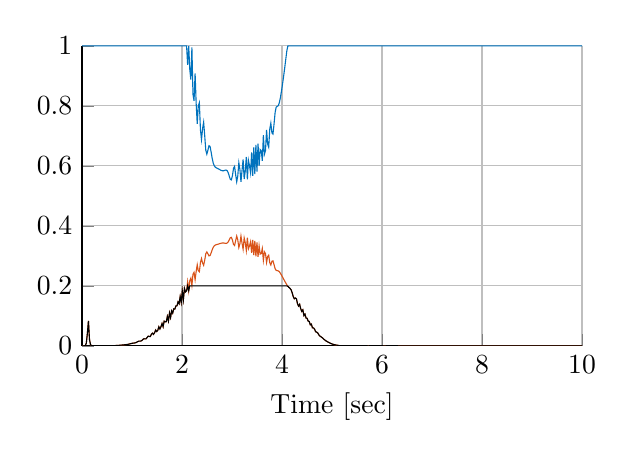
\begin{tikzpicture}

\begin{axis}[%
width=2.5in,
height=1.5in,
scale only axis,
xmin=0,
xmax=10,
xlabel={Time [sec]},
xmajorgrids,
ymin=0,
ymax=1,
ymajorgrids,
axis background/.style={fill=white},
axis x line*=bottom,
axis y line*=left
]
\addplot [color=mycolor1,solid,forget plot]
  table[row sep=crcr]{%
0	1\\
0.0213333333333333	1\\
0.0426666666666667	1\\
0.064	1\\
0.0853333333333333	1\\
0.106666666666667	1\\
0.128	1\\
0.149333333333333	1\\
0.170666666666667	1\\
0.192	1\\
0.213333333333333	1\\
0.234666666666667	1\\
0.256	1\\
0.277333333333333	1\\
0.298666666666667	1\\
0.32	1\\
0.341333333333333	1\\
0.362666666666667	1\\
0.384	1\\
0.405333333333333	1\\
0.426666666666667	1\\
0.448	1\\
0.469333333333333	1\\
0.490666666666667	1\\
0.512	1\\
0.533333333333333	1\\
0.554666666666667	1\\
0.576	1\\
0.597333333333333	1\\
0.618666666666667	1\\
0.64	1\\
0.661333333333333	1\\
0.682666666666667	1\\
0.704	1\\
0.725333333333333	1\\
0.746666666666667	1\\
0.768	1\\
0.789333333333333	1\\
0.810666666666667	1\\
0.832	1\\
0.853333333333333	1\\
0.874666666666667	1\\
0.896	1\\
0.917333333333333	1\\
0.938666666666667	1\\
0.96	1\\
0.981333333333333	1\\
1.00266666666667	1\\
1.024	1\\
1.04533333333333	1\\
1.06666666666667	1\\
1.088	1\\
1.10933333333333	1\\
1.13066666666667	1\\
1.152	1\\
1.17333333333333	1\\
1.19466666666667	1\\
1.216	1\\
1.23733333333333	1\\
1.25866666666667	1\\
1.28	1\\
1.30133333333333	1\\
1.32266666666667	1\\
1.344	1\\
1.36533333333333	1\\
1.38666666666667	1\\
1.408	1\\
1.42933333333333	1\\
1.45066666666667	1\\
1.472	1\\
1.49333333333333	1\\
1.51466666666667	1\\
1.536	1\\
1.55733333333333	1\\
1.57866666666667	1\\
1.6	1\\
1.62133333333333	1\\
1.64266666666667	1\\
1.664	1\\
1.68533333333333	1\\
1.70666666666667	1\\
1.728	1\\
1.74933333333333	1\\
1.77066666666667	1\\
1.792	1\\
1.81333333333333	1\\
1.83466666666667	1\\
1.856	1\\
1.87733333333333	1\\
1.89866666666667	1\\
1.92	1\\
1.94133333333333	1\\
1.96266666666667	1\\
1.984	1\\
2.00533333333333	1\\
2.02666666666667	1\\
2.048	1\\
2.06933333333333	1\\
2.09066666666667	1\\
2.112	0.936844508395851\\
2.13333333333333	1\\
2.15466666666667	0.921800216582387\\
2.176	0.887340381890603\\
2.19733333333333	0.994367208179842\\
2.21866666666667	0.838633796683989\\
2.24	0.816686576919312\\
2.26133333333333	0.907913932732287\\
2.28266666666667	0.807085960000964\\
2.304	0.740030231696991\\
2.32533333333333	0.799368869458874\\
2.34666666666667	0.810144697954745\\
2.368	0.719910723508446\\
2.38933333333333	0.687480711307636\\
2.41066666666667	0.723844583389203\\
2.432	0.745285508589601\\
2.45333333333333	0.70080291831211\\
2.47466666666667	0.652416541684589\\
2.496	0.6388984568693\\
2.51733333333333	0.652053634766654\\
2.53866666666667	0.667075178335245\\
2.56	0.664568193580873\\
2.58133333333333	0.646285705299739\\
2.60266666666667	0.625090091913308\\
2.624	0.609166149317089\\
2.64533333333333	0.599856551985683\\
2.66666666666667	0.595272549824847\\
2.688	0.593023968616242\\
2.70933333333333	0.59140217752156\\
2.73066666666667	0.58961245556373\\
2.752	0.587559959828053\\
2.77333333333333	0.585537386094231\\
2.79466666666667	0.583984107695834\\
2.816	0.583320303185968\\
2.83733333333333	0.58376437914191\\
2.85866666666667	0.585031477660997\\
2.88	0.585924908691039\\
2.90133333333333	0.584188731547631\\
2.92266666666667	0.577501740999613\\
2.944	0.566095718776544\\
2.96533333333333	0.555066880669894\\
2.98666666666667	0.553106656420884\\
3.008	0.567010726679938\\
3.02933333333333	0.591301575550618\\
3.05066666666667	0.598195539515138\\
3.072	0.570737829204805\\
3.09333333333333	0.546624557910814\\
3.11466666666667	0.566085587707771\\
3.136	0.61012574268765\\
3.15733333333333	0.587974056491266\\
3.17866666666667	0.546757377900598\\
3.2	0.584765824747783\\
3.22133333333333	0.620939349618024\\
3.24266666666667	0.556200356013283\\
3.264	0.581655911113395\\
3.28533333333333	0.629273235714636\\
3.30666666666667	0.554762247005058\\
3.328	0.618176096952403\\
3.34933333333333	0.600089945411984\\
3.37066666666667	0.576746085183146\\
3.392	0.644819783129468\\
3.41333333333333	0.56668196606594\\
3.43466666666667	0.661580839701769\\
3.456	0.572038573312345\\
3.47733333333333	0.669746097877421\\
3.49866666666667	0.580594951391407\\
3.52	0.673986683789032\\
3.54133333333333	0.599577378587408\\
3.56266666666667	0.654089762411656\\
3.584	0.650125695514627\\
3.60533333333333	0.616600231594588\\
3.62666666666667	0.701940784158025\\
3.648	0.638683576763388\\
3.66933333333333	0.650876029077659\\
3.69066666666667	0.719581038603853\\
3.712	0.672130469508098\\
3.73333333333333	0.662111854594971\\
3.75466666666667	0.722736243528206\\
3.776	0.742089645826732\\
3.79733333333333	0.709806745559987\\
3.81866666666667	0.705808673989911\\
3.84	0.739036829165959\\
3.86133333333333	0.777499153493558\\
3.88266666666667	0.795551596045662\\
3.904	0.798027293983414\\
3.92533333333333	0.80063499862328\\
3.94666666666667	0.81062924404324\\
3.968	0.827696003654507\\
3.98933333333333	0.849263368807239\\
4.01066666666667	0.873319543219653\\
4.032	0.899036765198172\\
4.05333333333333	0.926318080982512\\
4.07466666666667	0.954919409104426\\
4.096	0.983434398849123\\
4.11733333333333	1\\
4.13866666666667	1\\
4.16	1\\
4.18133333333333	1\\
4.20266666666667	1\\
4.224	1\\
4.24533333333333	1\\
4.26666666666667	1\\
4.288	1\\
4.30933333333333	1\\
4.33066666666667	1\\
4.352	1\\
4.37333333333333	1\\
4.39466666666667	1\\
4.416	1\\
4.43733333333333	1\\
4.45866666666667	1\\
4.48	1\\
4.50133333333333	1\\
4.52266666666667	1\\
4.544	1\\
4.56533333333333	1\\
4.58666666666667	1\\
4.608	1\\
4.62933333333333	1\\
4.65066666666667	1\\
4.672	1\\
4.69333333333333	1\\
4.71466666666667	1\\
4.736	1\\
4.75733333333333	1\\
4.77866666666667	1\\
4.8	1\\
4.82133333333333	1\\
4.84266666666667	1\\
4.864	1\\
4.88533333333333	1\\
4.90666666666667	1\\
4.928	1\\
4.94933333333333	1\\
4.97066666666667	1\\
4.992	1\\
5.01333333333333	1\\
5.03466666666667	1\\
5.056	1\\
5.07733333333333	1\\
5.09866666666667	1\\
5.12	1\\
5.14133333333333	1\\
5.16266666666667	1\\
5.184	1\\
5.20533333333333	1\\
5.22666666666667	1\\
5.248	1\\
5.26933333333333	1\\
5.29066666666667	1\\
5.312	1\\
5.33333333333333	1\\
5.35466666666667	1\\
5.376	1\\
5.39733333333333	1\\
5.41866666666667	1\\
5.44	1\\
5.46133333333333	1\\
5.48266666666667	1\\
5.504	1\\
5.52533333333333	1\\
5.54666666666667	1\\
5.568	1\\
5.58933333333333	1\\
5.61066666666667	1\\
5.632	1\\
5.65333333333333	1\\
5.67466666666667	1\\
5.696	1\\
5.71733333333333	1\\
5.73866666666667	1\\
5.76	1\\
5.78133333333333	1\\
5.80266666666667	1\\
5.824	1\\
5.84533333333333	1\\
5.86666666666667	1\\
5.888	1\\
5.90933333333333	1\\
5.93066666666667	1\\
5.952	1\\
5.97333333333333	1\\
5.99466666666667	1\\
6.016	1\\
6.03733333333333	1\\
6.05866666666667	1\\
6.08	1\\
6.10133333333333	1\\
6.12266666666667	1\\
6.144	1\\
6.16533333333333	1\\
6.18666666666667	1\\
6.208	1\\
6.22933333333333	1\\
6.25066666666667	1\\
6.272	1\\
6.29333333333333	1\\
6.31466666666667	1\\
6.336	1\\
6.35733333333333	1\\
6.37866666666667	1\\
6.4	1\\
6.42133333333333	1\\
6.44266666666667	1\\
6.464	1\\
6.48533333333333	1\\
6.50666666666667	1\\
6.528	1\\
6.54933333333333	1\\
6.57066666666667	1\\
6.592	1\\
6.61333333333333	1\\
6.63466666666667	1\\
6.656	1\\
6.67733333333333	1\\
6.69866666666667	1\\
6.72	1\\
6.74133333333333	1\\
6.76266666666667	1\\
6.784	1\\
6.80533333333333	1\\
6.82666666666667	1\\
6.848	1\\
6.86933333333333	1\\
6.89066666666667	1\\
6.912	1\\
6.93333333333333	1\\
6.95466666666667	1\\
6.976	1\\
6.99733333333333	1\\
7.01866666666667	1\\
7.04	1\\
7.06133333333333	1\\
7.08266666666667	1\\
7.104	1\\
7.12533333333333	1\\
7.14666666666667	1\\
7.168	1\\
7.18933333333333	1\\
7.21066666666667	1\\
7.232	1\\
7.25333333333333	1\\
7.27466666666667	1\\
7.296	1\\
7.31733333333333	1\\
7.33866666666667	1\\
7.36	1\\
7.38133333333333	1\\
7.40266666666667	1\\
7.424	1\\
7.44533333333333	1\\
7.46666666666667	1\\
7.488	1\\
7.50933333333333	1\\
7.53066666666667	1\\
7.552	1\\
7.57333333333333	1\\
7.59466666666667	1\\
7.616	1\\
7.63733333333333	1\\
7.65866666666667	1\\
7.68	1\\
7.70133333333333	1\\
7.72266666666667	1\\
7.744	1\\
7.76533333333333	1\\
7.78666666666667	1\\
7.808	1\\
7.82933333333333	1\\
7.85066666666667	1\\
7.872	1\\
7.89333333333333	1\\
7.91466666666667	1\\
7.936	1\\
7.95733333333333	1\\
7.97866666666667	1\\
8	1\\
8.02133333333333	1\\
8.04266666666667	1\\
8.064	1\\
8.08533333333333	1\\
8.10666666666667	1\\
8.128	1\\
8.14933333333333	1\\
8.17066666666667	1\\
8.192	1\\
8.21333333333333	1\\
8.23466666666667	1\\
8.256	1\\
8.27733333333333	1\\
8.29866666666667	1\\
8.32	1\\
8.34133333333333	1\\
8.36266666666667	1\\
8.384	1\\
8.40533333333333	1\\
8.42666666666667	1\\
8.448	1\\
8.46933333333333	1\\
8.49066666666667	1\\
8.512	1\\
8.53333333333333	1\\
8.55466666666667	1\\
8.576	1\\
8.59733333333333	1\\
8.61866666666667	1\\
8.64	1\\
8.66133333333333	1\\
8.68266666666667	1\\
8.704	1\\
8.72533333333333	1\\
8.74666666666667	1\\
8.768	1\\
8.78933333333333	1\\
8.81066666666667	1\\
8.832	1\\
8.85333333333333	1\\
8.87466666666667	1\\
8.896	1\\
8.91733333333333	1\\
8.93866666666667	1\\
8.96	1\\
8.98133333333333	1\\
9.00266666666667	1\\
9.024	1\\
9.04533333333333	1\\
9.06666666666667	1\\
9.088	1\\
9.10933333333333	1\\
9.13066666666667	1\\
9.152	1\\
9.17333333333333	1\\
9.19466666666667	1\\
9.216	1\\
9.23733333333333	1\\
9.25866666666667	1\\
9.28	1\\
9.30133333333333	1\\
9.32266666666667	1\\
9.344	1\\
9.36533333333333	1\\
9.38666666666667	1\\
9.408	1\\
9.42933333333333	1\\
9.45066666666667	1\\
9.472	1\\
9.49333333333333	1\\
9.51466666666667	1\\
9.536	1\\
9.55733333333333	1\\
9.57866666666667	1\\
9.6	1\\
9.62133333333333	1\\
9.64266666666667	1\\
9.664	1\\
9.68533333333333	1\\
9.70666666666667	1\\
9.728	1\\
9.74933333333333	1\\
9.77066666666667	1\\
9.792	1\\
9.81333333333333	1\\
9.83466666666667	1\\
9.856	1\\
9.87733333333333	1\\
9.89866666666667	1\\
9.92	1\\
9.94133333333333	1\\
9.96266666666667	1\\
9.984	1\\
10.0053333333333	1\\
};
\addplot [color=mycolor2,solid,forget plot]
  table[row sep=crcr]{%
0	1.37398031960227e-12\\
0.0213333333333333	1.73091567005322e-07\\
0.0426666666666667	7.1898284287654e-06\\
0.064	0.000589380586125306\\
0.0853333333333333	0.00844686672802343\\
0.106666666666667	0.0408881668467508\\
0.128	0.082989352050691\\
0.149333333333333	0.0203334673382813\\
0.170666666666667	0.00344859168960224\\
0.192	0.000373171573493537\\
0.213333333333333	0.000299856121485226\\
0.234666666666667	0.000309275620741836\\
0.256	0.000323778263066804\\
0.277333333333333	0.000345345179033911\\
0.298666666666667	0.000369857916217054\\
0.32	0.000391911446440857\\
0.341333333333333	0.00040761042160201\\
0.362666666666667	0.00041533209993261\\
0.384	0.000415259294843679\\
0.405333333333333	0.000408551197299379\\
0.426666666666667	0.000396636578552113\\
0.448	0.000380853621278948\\
0.469333333333333	0.000362511331996073\\
0.490666666666667	0.000343363767417923\\
0.512	0.00032644037311345\\
0.533333333333333	0.000317017822562046\\
0.554666666666667	0.000322928571630694\\
0.576	0.000352758585976015\\
0.597333333333333	0.000412335524795413\\
0.618666666666667	0.000503370597034906\\
0.64	0.000625512183726147\\
0.661333333333333	0.0007786339425054\\
0.682666666666667	0.000963638563842606\\
0.704	0.0011822010341944\\
0.725333333333333	0.00143595721818584\\
0.746666666666667	0.00172530381368775\\
0.768	0.00204795516375265\\
0.789333333333333	0.00239768286382574\\
0.810666666666667	0.00276416973812268\\
0.832	0.00313554012484005\\
0.853333333333333	0.00350551467803186\\
0.874666666666667	0.00388603335033514\\
0.896	0.00432069952275699\\
0.917333333333333	0.00488271069004835\\
0.938666666666667	0.00563613117727873\\
0.96	0.00657035965995725\\
0.981333333333333	0.00756289899793415\\
1.00266666666667	0.00841628466533676\\
1.024	0.00898030785204012\\
1.04533333333333	0.00935233533632151\\
1.06666666666667	0.0100216573043312\\
1.088	0.0115148922423224\\
1.10933333333333	0.0135951166699649\\
1.13066666666667	0.0152726584197823\\
1.152	0.0157732279553585\\
1.17333333333333	0.0157279296118817\\
1.19466666666667	0.0173176736601007\\
1.216	0.0208889351890108\\
1.23733333333333	0.0234745271346318\\
1.25866666666667	0.0231286696661288\\
1.28	0.0229903681145226\\
1.30133333333333	0.0276040076615383\\
1.32266666666667	0.0322324105533992\\
1.344	0.0312817998786315\\
1.36533333333333	0.0307106051989484\\
1.38666666666667	0.0382104518432329\\
1.408	0.0421430513391746\\
1.42933333333333	0.0381069865306387\\
1.45066666666667	0.0436562673145006\\
1.472	0.0525223959510886\\
1.49333333333333	0.0475615470279882\\
1.51466666666667	0.0516102940500722\\
1.536	0.0634654609521921\\
1.55733333333333	0.0561476561680924\\
1.57866666666667	0.0639236109172942\\
1.6	0.0744854817633786\\
1.62133333333333	0.0638733155496329\\
1.64266666666667	0.0822284765887533\\
1.664	0.0800250914526096\\
1.68533333333333	0.0804546845399198\\
1.70666666666667	0.0981266950431886\\
1.728	0.0829316956515217\\
1.74933333333333	0.109476813432823\\
1.77066666666667	0.0942289934471908\\
1.792	0.11635483879262\\
1.81333333333333	0.108943768708274\\
1.83466666666667	0.123213161248519\\
1.856	0.122572483441772\\
1.87733333333333	0.132874561014256\\
1.89866666666667	0.13331212236005\\
1.92	0.146597672975364\\
1.94133333333333	0.140301279438552\\
1.96266666666667	0.16429123248829\\
1.984	0.144482702219015\\
2.00533333333333	0.182333098055378\\
2.02666666666667	0.153497770228778\\
2.048	0.191111689682657\\
2.06933333333333	0.179778189855067\\
2.09066666666667	0.183090306555221\\
2.112	0.213482598454313\\
2.13333333333333	0.183710190038037\\
2.15466666666667	0.216966753101348\\
2.176	0.225392649857625\\
2.19733333333333	0.201132939979079\\
2.21866666666667	0.238483114788377\\
2.24	0.244891988741184\\
2.26133333333333	0.220285197516595\\
2.28266666666667	0.247805078903567\\
2.304	0.270259229195776\\
2.32533333333333	0.250197384012951\\
2.34666666666667	0.246869479618778\\
2.368	0.27781222513996\\
2.38933333333333	0.290917252964939\\
2.41066666666667	0.276302406054564\\
2.432	0.268353533907409\\
2.45333333333333	0.285386939428993\\
2.47466666666667	0.306552619716822\\
2.496	0.313038790201546\\
2.51733333333333	0.30672323461792\\
2.53866666666667	0.299816282325361\\
2.56	0.300947294697247\\
2.58133333333333	0.30946065859099\\
2.60266666666667	0.319953879588508\\
2.624	0.328317652292748\\
2.64533333333333	0.333413045732263\\
2.66666666666667	0.335980552200581\\
2.688	0.337254496587513\\
2.70933333333333	0.338179343265453\\
2.73066666666667	0.339205859904672\\
2.752	0.340390791875146\\
2.77333333333333	0.341566575849375\\
2.79466666666667	0.342475073147315\\
2.816	0.342864801563812\\
2.83733333333333	0.342603980554595\\
2.85866666666667	0.341861946983804\\
2.88	0.341340668460062\\
2.90133333333333	0.342355114365456\\
2.92266666666667	0.346319302265331\\
2.944	0.353297142808717\\
2.96533333333333	0.360316940111119\\
2.98666666666667	0.361593912635561\\
3.008	0.35272701306918\\
3.02933333333333	0.338236879909817\\
3.05066666666667	0.334338835361608\\
3.072	0.350423591649173\\
3.09333333333333	0.365881841760632\\
3.11466666666667	0.353303465664711\\
3.136	0.32780128096052\\
3.15733333333333	0.340151062435475\\
3.17866666666667	0.365792960614352\\
3.2	0.342017251241149\\
3.22133333333333	0.322092649021248\\
3.24266666666667	0.359582653692555\\
3.264	0.343845899575169\\
3.28533333333333	0.317826960768274\\
3.30666666666667	0.360514799050802\\
3.328	0.323532406034456\\
3.34933333333333	0.333283371149791\\
3.37066666666667	0.346773051674014\\
3.392	0.310164181113289\\
3.41333333333333	0.352931647690246\\
3.43466666666667	0.302306215654851\\
3.456	0.349626772268023\\
3.47733333333333	0.298620627479347\\
3.49866666666667	0.344474232028191\\
3.52	0.29674176776852\\
3.54133333333333	0.333568288502138\\
3.56266666666667	0.305768430410211\\
3.584	0.307632818360892\\
3.60533333333333	0.324359268375201\\
3.62666666666667	0.284924319135978\\
3.648	0.313144109659945\\
3.66933333333333	0.30727817751011\\
3.69066666666667	0.27793950822835\\
3.712	0.297561275783809\\
3.73333333333333	0.302063765528476\\
3.75466666666667	0.27672612490506\\
3.776	0.269509217821235\\
3.79733333333333	0.28176683477728\\
3.81866666666667	0.28336291033292\\
3.84	0.270622507711436\\
3.86133333333333	0.257235006753814\\
3.88266666666667	0.251397899261484\\
3.904	0.250617994532098\\
3.92533333333333	0.249801720314384\\
3.94666666666667	0.246721915684221\\
3.968	0.241634608741548\\
3.98933333333333	0.235498206264204\\
4.01066666666667	0.229011249722711\\
4.032	0.222460312794788\\
4.05333333333333	0.215908556797107\\
4.07466666666667	0.209441758218707\\
4.096	0.203368928556956\\
4.11733333333333	0.198255635152723\\
4.13866666666667	0.194521327051921\\
4.16	0.19146730256592\\
4.18133333333333	0.186561617681481\\
4.20266666666667	0.17695239331752\\
4.224	0.164177368506176\\
4.24533333333333	0.156978829009594\\
4.26666666666667	0.159270186751945\\
4.288	0.156750806760155\\
4.30933333333333	0.140309695768544\\
4.33066666666667	0.132600123158329\\
4.352	0.138271902335026\\
4.37333333333333	0.123899912230395\\
4.39466666666667	0.114841792584637\\
4.416	0.119797120600858\\
4.43733333333333	0.100839370610191\\
4.45866666666667	0.10561138835266\\
4.48	0.0926579482612482\\
4.50133333333333	0.0917372466871695\\
4.52266666666667	0.0822760958911304\\
4.544	0.0812933158448369\\
4.56533333333333	0.0699293655903125\\
4.58666666666667	0.0722738604706564\\
4.608	0.0597779084343281\\
4.62933333333333	0.0598060321358616\\
4.65066666666667	0.0554165846933687\\
4.672	0.046787241512002\\
4.69333333333333	0.045732681385251\\
4.71466666666667	0.0428223289954852\\
4.736	0.0366041623490636\\
4.75733333333333	0.0323161143707478\\
4.77866666666667	0.0301046802029765\\
4.8	0.0276110843251502\\
4.82133333333333	0.0244146770944571\\
4.84266666666667	0.0211644134058168\\
4.864	0.0182885677835797\\
4.88533333333333	0.0158205166682277\\
4.90666666666667	0.0136505355354012\\
4.928	0.0116903322448039\\
4.94933333333333	0.00989752248289416\\
4.97066666666667	0.00825521489153897\\
4.992	0.00676196089196597\\
5.01333333333333	0.00543855045517\\
5.03466666666667	0.0043277290754342\\
5.056	0.00344705561073859\\
5.07733333333333	0.00271885290166487\\
5.09866666666667	0.00202351965368202\\
5.12	0.00137079919380636\\
5.14133333333333	0.000898044297007735\\
5.16266666666667	0.000620956228515686\\
5.184	0.000453385919318697\\
5.20533333333333	0.000401552185727585\\
5.22666666666667	0.000395893415055334\\
5.248	0.00042030966800866\\
5.26933333333333	0.000459056863051518\\
5.29066666666667	0.00039120430027696\\
5.312	0.000396959036385534\\
5.33333333333333	0.000295274438464938\\
5.35466666666667	0.000253548640224016\\
5.376	0.000160041058334942\\
5.39733333333333	8.79224288417425e-05\\
5.41866666666667	3.773631668227e-05\\
5.44	8.63479649481946e-05\\
5.46133333333333	0.000133998599942228\\
5.48266666666667	0.000182182258179981\\
5.504	0.000230237703025726\\
5.52533333333333	0.000257527935870273\\
5.54666666666667	0.000264195767033751\\
5.568	0.000258538474273078\\
5.58933333333333	0.000244348370233392\\
5.61066666666667	0.000221782856398741\\
5.632	0.000190916913866608\\
5.65333333333333	0.000152829202319648\\
5.67466666666667	0.000109722346654405\\
5.696	6.54820547928398e-05\\
5.71733333333333	2.63247049326663e-05\\
5.73866666666667	2.62608828787915e-05\\
5.76	6.52165933451192e-05\\
5.78133333333333	9.87732989653648e-05\\
5.80266666666667	0.00011615406293349\\
5.824	0.000146210188034922\\
5.84533333333333	0.000162751314655721\\
5.86666666666667	0.000151507225901178\\
5.888	0.000172218504880261\\
5.90933333333333	0.000140871394040783\\
5.93066666666667	0.000147686332260315\\
5.952	0.000109193451336948\\
5.97333333333333	0.000101019196762304\\
5.99466666666667	6.77492776191144e-05\\
6.016	4.18965140306219e-05\\
6.03733333333333	2.01923365162466e-05\\
6.05866666666667	1.68143887320612e-05\\
6.08	3.66227290903915e-05\\
6.10133333333333	5.26945265308178e-05\\
6.12266666666667	6.82601533026977e-05\\
6.144	8.1046597279057e-05\\
6.16533333333333	8.86858841935871e-05\\
6.18666666666667	9.109313850033e-05\\
6.208	8.92795100247616e-05\\
6.22933333333333	8.44846182204833e-05\\
6.25066666666667	7.7256661253264e-05\\
6.272	6.6350971471956e-05\\
6.29333333333333	5.060443675184e-05\\
6.31466666666667	3.45839255437146e-05\\
6.336	2.41793852703471e-05\\
6.35733333333333	1.36964573238048e-05\\
6.37866666666667	7.48629579801403e-06\\
6.4	1.44802636775851e-05\\
6.42133333333333	1.78948608461131e-05\\
6.44266666666667	2.63290608403745e-05\\
6.464	2.3961396836453e-05\\
6.48533333333333	2.98389812827268e-05\\
6.50666666666667	2.31118255544821e-05\\
6.528	2.15128737089628e-05\\
6.54933333333333	1.90857855904018e-05\\
6.57066666666667	1.19135341670446e-05\\
6.592	6.16397765517804e-06\\
6.61333333333333	3.09944662225182e-06\\
6.63466666666667	4.16285035418143e-06\\
6.656	7.61903326373613e-06\\
6.67733333333333	1.0814132864735e-05\\
6.69866666666667	1.32583016527214e-05\\
6.72	1.45794766921995e-05\\
6.74133333333333	1.38462786958546e-05\\
6.76266666666667	1.09866707629449e-05\\
6.784	1.00863932273825e-05\\
6.80533333333333	1.05597833932727e-05\\
6.82666666666667	6.15251430009369e-06\\
6.848	4.16510492664463e-06\\
6.86933333333333	3.30563694235008e-06\\
6.89066666666667	1.31849238040113e-06\\
6.912	1.09637633961692e-06\\
6.93333333333333	2.62470340600596e-06\\
6.95466666666667	1.61606834400769e-06\\
6.976	1.86184796568957e-06\\
6.99733333333333	2.95260032120347e-06\\
7.01866666666667	2.28848492689934e-06\\
7.04	1.12251536578163e-06\\
7.06133333333333	2.9333364958753e-07\\
7.08266666666667	2.22850739354149e-07\\
7.104	4.6101077197575e-07\\
7.12533333333333	6.63303699412223e-07\\
7.14666666666667	7.62157697283813e-07\\
7.168	5.86606793674401e-07\\
7.18933333333333	1.82469513708401e-07\\
7.21066666666667	4.04223768594035e-07\\
7.232	4.11916744583454e-07\\
7.25333333333333	1.23684361404957e-07\\
7.27466666666667	1.42107540794006e-07\\
7.296	1.1389012354921e-07\\
7.31733333333333	6.47939032941216e-08\\
7.33866666666667	5.00904738692626e-08\\
7.36	2.74641720806742e-08\\
7.38133333333333	3.52257613117116e-08\\
7.40266666666667	5.7431497654947e-08\\
7.424	7.8416841815916e-08\\
7.44533333333333	8.67622162887503e-08\\
7.46666666666667	8.14768811927657e-08\\
7.488	6.73096005329793e-08\\
7.50933333333333	4.90621853982863e-08\\
7.53066666666667	3.23727288732063e-08\\
7.552	2.19536406001578e-08\\
7.57333333333333	1.51332120545484e-08\\
7.59466666666667	1.21941551956152e-08\\
7.616	5.64911908101078e-09\\
7.63733333333333	6.75976311543061e-09\\
7.65866666666667	1.30112071361585e-08\\
7.68	1.46964816663566e-08\\
7.70133333333333	1.10596875941877e-08\\
7.72266666666667	6.26824592902611e-09\\
7.744	2.77676566504013e-09\\
7.76533333333333	9.56064967872177e-09\\
7.78666666666667	1.47456617949393e-08\\
7.808	1.66093042647639e-08\\
7.82933333333333	1.48618659448536e-08\\
7.85066666666667	9.63958289151775e-09\\
7.872	4.14201338658963e-09\\
7.89333333333333	5.04652553317388e-09\\
7.91466666666667	7.04116956088604e-09\\
7.936	8.37298471556483e-09\\
7.95733333333333	5.92886104803031e-09\\
7.97866666666667	3.53680617867314e-09\\
8	2.32366303956331e-09\\
8.02133333333333	3.98338327111879e-09\\
8.04266666666667	4.18606563869384e-09\\
8.064	2.96655042809132e-09\\
8.08533333333333	9.26290680769498e-10\\
8.10666666666667	2.35687316182351e-09\\
8.128	3.81411959195749e-09\\
8.14933333333333	3.87998349643129e-09\\
8.17066666666667	2.99497772028865e-09\\
8.192	1.35165556306872e-09\\
8.21333333333333	2.22242635721255e-09\\
8.23466666666667	2.97479471337954e-09\\
8.256	2.92620838282246e-09\\
8.27733333333333	2.98608914243144e-09\\
8.29866666666667	4.95157374044934e-09\\
8.32	7.65740265763224e-09\\
8.34133333333333	9.57335814422743e-09\\
8.36266666666667	9.83914913715235e-09\\
8.384	8.14850367783613e-09\\
8.40533333333333	5.03374534551108e-09\\
8.42666666666667	2.51163081865835e-09\\
8.448	2.58223490863168e-09\\
8.46933333333333	3.29108685886125e-09\\
8.49066666666667	3.05585743039899e-09\\
8.512	1.61951836739183e-09\\
8.53333333333333	8.35431226766404e-10\\
8.55466666666667	1.73749055253409e-09\\
8.576	2.19385998405108e-09\\
8.59733333333333	1.74033326380844e-09\\
8.61866666666667	6.95158767798486e-10\\
8.64	9.52805218518485e-10\\
8.66133333333333	1.59701799707493e-09\\
8.68266666666667	1.80055706056673e-09\\
8.704	1.53183223310898e-09\\
8.72533333333333	9.20871680444359e-10\\
8.74666666666667	8.95994975247922e-10\\
8.768	6.92303317429592e-10\\
8.78933333333333	4.93100532529731e-10\\
8.81066666666667	5.76027600125746e-10\\
8.832	7.72782384030069e-10\\
8.85333333333333	7.41877729405516e-10\\
8.87466666666667	5.28847708254613e-10\\
8.896	3.31358944054394e-10\\
8.91733333333333	3.51606667656421e-10\\
8.93866666666667	3.74801527268781e-10\\
8.96	2.47355780617855e-10\\
8.98133333333333	1.99593471262594e-10\\
9.00266666666667	9.04065574894304e-11\\
9.024	5.04772699116937e-11\\
9.04533333333333	2.45091619716099e-11\\
9.06666666666667	8.30495244964277e-12\\
9.088	3.3109708503392e-12\\
9.10933333333333	1.51679889575697e-12\\
9.13066666666667	6.09834722079594e-13\\
9.152	2.24106894914013e-13\\
9.17333333333333	8.93312765874836e-14\\
9.19466666666667	6.6946490764745e-14\\
9.216	7.58742064287412e-14\\
9.23733333333333	6.5767250079739e-14\\
9.25866666666667	5.37934593442762e-14\\
9.28	9.75851709006248e-15\\
9.30133333333333	9.036567461935e-15\\
9.32266666666667	2.65534970308944e-14\\
9.344	3.96619706926544e-14\\
9.36533333333333	5.70223957880395e-14\\
9.38666666666667	1.20593021747828e-13\\
9.408	1.90833324053358e-13\\
9.42933333333333	3.08712823278902e-13\\
9.45066666666667	4.29696262767839e-13\\
9.472	8.16213652633834e-13\\
9.49333333333333	1.34047672218079e-12\\
9.51466666666667	2.18333885393671e-12\\
9.536	3.38234326906537e-12\\
9.55733333333333	4.79552554223495e-12\\
9.57866666666667	6.02498037809173e-12\\
9.6	6.05119926484928e-12\\
9.62133333333333	4.23637226067131e-12\\
9.64266666666667	2.88834472818913e-12\\
9.664	3.00469449495629e-12\\
9.68533333333333	2.70948090662246e-12\\
9.70666666666667	1.85118011459747e-12\\
9.728	8.82649651197715e-13\\
9.74933333333333	8.07063051826181e-13\\
9.77066666666667	1.2876331624023e-12\\
9.792	1.36102340307409e-12\\
9.81333333333333	1.58889584541925e-12\\
9.83466666666667	1.13836216831599e-12\\
9.856	1.01102756743367e-12\\
9.87733333333333	1.21105470401486e-12\\
9.89866666666667	5.83796649972481e-13\\
9.92	8.1338826667834e-13\\
9.94133333333333	9.19451474831784e-13\\
9.96266666666667	4.51076023587096e-13\\
9.984	6.45203067052932e-13\\
10.0053333333333	5.64034640873646e-11\\
};
\addplot [color=mycolor3,solid,forget plot]
  table[row sep=crcr]{%
0	1.37398031960227e-12\\
0.0213333333333333	1.73091567005322e-07\\
0.0426666666666667	7.1898284287654e-06\\
0.064	0.000589380586125306\\
0.0853333333333333	0.00844686672802343\\
0.106666666666667	0.0408881668467508\\
0.128	0.082989352050691\\
0.149333333333333	0.0203334673382813\\
0.170666666666667	0.00344859168960224\\
0.192	0.000373171573493537\\
0.213333333333333	0.000299856121485226\\
0.234666666666667	0.000309275620741836\\
0.256	0.000323778263066804\\
0.277333333333333	0.000345345179033911\\
0.298666666666667	0.000369857916217054\\
0.32	0.000391911446440857\\
0.341333333333333	0.00040761042160201\\
0.362666666666667	0.00041533209993261\\
0.384	0.000415259294843679\\
0.405333333333333	0.000408551197299379\\
0.426666666666667	0.000396636578552113\\
0.448	0.000380853621278948\\
0.469333333333333	0.000362511331996073\\
0.490666666666667	0.000343363767417923\\
0.512	0.00032644037311345\\
0.533333333333333	0.000317017822562046\\
0.554666666666667	0.000322928571630694\\
0.576	0.000352758585976015\\
0.597333333333333	0.000412335524795413\\
0.618666666666667	0.000503370597034906\\
0.64	0.000625512183726147\\
0.661333333333333	0.0007786339425054\\
0.682666666666667	0.000963638563842606\\
0.704	0.0011822010341944\\
0.725333333333333	0.00143595721818584\\
0.746666666666667	0.00172530381368775\\
0.768	0.00204795516375265\\
0.789333333333333	0.00239768286382574\\
0.810666666666667	0.00276416973812268\\
0.832	0.00313554012484005\\
0.853333333333333	0.00350551467803186\\
0.874666666666667	0.00388603335033514\\
0.896	0.00432069952275699\\
0.917333333333333	0.00488271069004835\\
0.938666666666667	0.00563613117727873\\
0.96	0.00657035965995725\\
0.981333333333333	0.00756289899793415\\
1.00266666666667	0.00841628466533676\\
1.024	0.00898030785204012\\
1.04533333333333	0.00935233533632151\\
1.06666666666667	0.0100216573043312\\
1.088	0.0115148922423224\\
1.10933333333333	0.0135951166699649\\
1.13066666666667	0.0152726584197823\\
1.152	0.0157732279553585\\
1.17333333333333	0.0157279296118817\\
1.19466666666667	0.0173176736601007\\
1.216	0.0208889351890108\\
1.23733333333333	0.0234745271346318\\
1.25866666666667	0.0231286696661288\\
1.28	0.0229903681145226\\
1.30133333333333	0.0276040076615383\\
1.32266666666667	0.0322324105533992\\
1.344	0.0312817998786315\\
1.36533333333333	0.0307106051989484\\
1.38666666666667	0.0382104518432329\\
1.408	0.0421430513391746\\
1.42933333333333	0.0381069865306387\\
1.45066666666667	0.0436562673145006\\
1.472	0.0525223959510886\\
1.49333333333333	0.0475615470279882\\
1.51466666666667	0.0516102940500722\\
1.536	0.0634654609521921\\
1.55733333333333	0.0561476561680924\\
1.57866666666667	0.0639236109172942\\
1.6	0.0744854817633786\\
1.62133333333333	0.0638733155496329\\
1.64266666666667	0.0822284765887533\\
1.664	0.0800250914526096\\
1.68533333333333	0.0804546845399198\\
1.70666666666667	0.0981266950431886\\
1.728	0.0829316956515217\\
1.74933333333333	0.109476813432823\\
1.77066666666667	0.0942289934471908\\
1.792	0.11635483879262\\
1.81333333333333	0.108943768708274\\
1.83466666666667	0.123213161248519\\
1.856	0.122572483441772\\
1.87733333333333	0.132874561014256\\
1.89866666666667	0.13331212236005\\
1.92	0.146597672975364\\
1.94133333333333	0.140301279438552\\
1.96266666666667	0.16429123248829\\
1.984	0.144482702219015\\
2.00533333333333	0.182333098055378\\
2.02666666666667	0.153497770228778\\
2.048	0.191111689682657\\
2.06933333333333	0.179778189855067\\
2.09066666666667	0.183090306555221\\
2.112	0.2\\
2.13333333333333	0.183710190038037\\
2.15466666666667	0.2\\
2.176	0.2\\
2.19733333333333	0.2\\
2.21866666666667	0.2\\
2.24	0.2\\
2.26133333333333	0.2\\
2.28266666666667	0.2\\
2.304	0.2\\
2.32533333333333	0.2\\
2.34666666666667	0.2\\
2.368	0.2\\
2.38933333333333	0.2\\
2.41066666666667	0.2\\
2.432	0.2\\
2.45333333333333	0.2\\
2.47466666666667	0.2\\
2.496	0.2\\
2.51733333333333	0.2\\
2.53866666666667	0.2\\
2.56	0.2\\
2.58133333333333	0.2\\
2.60266666666667	0.2\\
2.624	0.2\\
2.64533333333333	0.2\\
2.66666666666667	0.2\\
2.688	0.2\\
2.70933333333333	0.2\\
2.73066666666667	0.2\\
2.752	0.2\\
2.77333333333333	0.2\\
2.79466666666667	0.2\\
2.816	0.2\\
2.83733333333333	0.2\\
2.85866666666667	0.2\\
2.88	0.2\\
2.90133333333333	0.2\\
2.92266666666667	0.2\\
2.944	0.2\\
2.96533333333333	0.2\\
2.98666666666667	0.2\\
3.008	0.2\\
3.02933333333333	0.2\\
3.05066666666667	0.2\\
3.072	0.2\\
3.09333333333333	0.2\\
3.11466666666667	0.2\\
3.136	0.2\\
3.15733333333333	0.2\\
3.17866666666667	0.2\\
3.2	0.2\\
3.22133333333333	0.2\\
3.24266666666667	0.2\\
3.264	0.2\\
3.28533333333333	0.2\\
3.30666666666667	0.2\\
3.328	0.2\\
3.34933333333333	0.2\\
3.37066666666667	0.2\\
3.392	0.2\\
3.41333333333333	0.2\\
3.43466666666667	0.2\\
3.456	0.2\\
3.47733333333333	0.2\\
3.49866666666667	0.2\\
3.52	0.2\\
3.54133333333333	0.2\\
3.56266666666667	0.2\\
3.584	0.2\\
3.60533333333333	0.2\\
3.62666666666667	0.2\\
3.648	0.2\\
3.66933333333333	0.2\\
3.69066666666667	0.2\\
3.712	0.2\\
3.73333333333333	0.2\\
3.75466666666667	0.2\\
3.776	0.2\\
3.79733333333333	0.2\\
3.81866666666667	0.2\\
3.84	0.2\\
3.86133333333333	0.2\\
3.88266666666667	0.2\\
3.904	0.2\\
3.92533333333333	0.2\\
3.94666666666667	0.2\\
3.968	0.2\\
3.98933333333333	0.2\\
4.01066666666667	0.2\\
4.032	0.2\\
4.05333333333333	0.2\\
4.07466666666667	0.2\\
4.096	0.2\\
4.11733333333333	0.198255635152723\\
4.13866666666667	0.194521327051921\\
4.16	0.19146730256592\\
4.18133333333333	0.186561617681481\\
4.20266666666667	0.17695239331752\\
4.224	0.164177368506176\\
4.24533333333333	0.156978829009594\\
4.26666666666667	0.159270186751945\\
4.288	0.156750806760155\\
4.30933333333333	0.140309695768544\\
4.33066666666667	0.132600123158329\\
4.352	0.138271902335026\\
4.37333333333333	0.123899912230395\\
4.39466666666667	0.114841792584637\\
4.416	0.119797120600858\\
4.43733333333333	0.100839370610191\\
4.45866666666667	0.10561138835266\\
4.48	0.0926579482612482\\
4.50133333333333	0.0917372466871695\\
4.52266666666667	0.0822760958911304\\
4.544	0.0812933158448369\\
4.56533333333333	0.0699293655903125\\
4.58666666666667	0.0722738604706564\\
4.608	0.0597779084343281\\
4.62933333333333	0.0598060321358616\\
4.65066666666667	0.0554165846933687\\
4.672	0.046787241512002\\
4.69333333333333	0.045732681385251\\
4.71466666666667	0.0428223289954852\\
4.736	0.0366041623490636\\
4.75733333333333	0.0323161143707478\\
4.77866666666667	0.0301046802029765\\
4.8	0.0276110843251502\\
4.82133333333333	0.0244146770944571\\
4.84266666666667	0.0211644134058168\\
4.864	0.0182885677835797\\
4.88533333333333	0.0158205166682277\\
4.90666666666667	0.0136505355354012\\
4.928	0.0116903322448039\\
4.94933333333333	0.00989752248289416\\
4.97066666666667	0.00825521489153897\\
4.992	0.00676196089196597\\
5.01333333333333	0.00543855045517\\
5.03466666666667	0.0043277290754342\\
5.056	0.00344705561073859\\
5.07733333333333	0.00271885290166487\\
5.09866666666667	0.00202351965368202\\
5.12	0.00137079919380636\\
5.14133333333333	0.000898044297007735\\
5.16266666666667	0.000620956228515686\\
5.184	0.000453385919318697\\
5.20533333333333	0.000401552185727585\\
5.22666666666667	0.000395893415055334\\
5.248	0.00042030966800866\\
5.26933333333333	0.000459056863051518\\
5.29066666666667	0.00039120430027696\\
5.312	0.000396959036385534\\
5.33333333333333	0.000295274438464938\\
5.35466666666667	0.000253548640224016\\
5.376	0.000160041058334942\\
5.39733333333333	8.79224288417425e-05\\
5.41866666666667	3.773631668227e-05\\
5.44	8.63479649481946e-05\\
5.46133333333333	0.000133998599942228\\
5.48266666666667	0.000182182258179981\\
5.504	0.000230237703025726\\
5.52533333333333	0.000257527935870273\\
5.54666666666667	0.000264195767033751\\
5.568	0.000258538474273078\\
5.58933333333333	0.000244348370233392\\
5.61066666666667	0.000221782856398741\\
5.632	0.000190916913866608\\
5.65333333333333	0.000152829202319648\\
5.67466666666667	0.000109722346654405\\
5.696	6.54820547928398e-05\\
5.71733333333333	2.63247049326663e-05\\
5.73866666666667	2.62608828787915e-05\\
5.76	6.52165933451192e-05\\
5.78133333333333	9.87732989653648e-05\\
5.80266666666667	0.00011615406293349\\
5.824	0.000146210188034922\\
5.84533333333333	0.000162751314655721\\
5.86666666666667	0.000151507225901178\\
5.888	0.000172218504880261\\
5.90933333333333	0.000140871394040783\\
5.93066666666667	0.000147686332260315\\
5.952	0.000109193451336948\\
5.97333333333333	0.000101019196762304\\
5.99466666666667	6.77492776191144e-05\\
6.016	4.18965140306219e-05\\
6.03733333333333	2.01923365162466e-05\\
6.05866666666667	1.68143887320612e-05\\
6.08	3.66227290903915e-05\\
6.10133333333333	5.26945265308178e-05\\
6.12266666666667	6.82601533026977e-05\\
6.144	8.1046597279057e-05\\
6.16533333333333	8.86858841935871e-05\\
6.18666666666667	9.109313850033e-05\\
6.208	8.92795100247616e-05\\
6.22933333333333	8.44846182204833e-05\\
6.25066666666667	7.7256661253264e-05\\
6.272	6.6350971471956e-05\\
6.29333333333333	5.060443675184e-05\\
6.31466666666667	3.45839255437146e-05\\
6.336	2.41793852703471e-05\\
6.35733333333333	1.36964573238048e-05\\
6.37866666666667	7.48629579801403e-06\\
6.4	1.44802636775851e-05\\
6.42133333333333	1.78948608461131e-05\\
6.44266666666667	2.63290608403745e-05\\
6.464	2.3961396836453e-05\\
6.48533333333333	2.98389812827268e-05\\
6.50666666666667	2.31118255544821e-05\\
6.528	2.15128737089628e-05\\
6.54933333333333	1.90857855904018e-05\\
6.57066666666667	1.19135341670446e-05\\
6.592	6.16397765517804e-06\\
6.61333333333333	3.09944662225182e-06\\
6.63466666666667	4.16285035418143e-06\\
6.656	7.61903326373613e-06\\
6.67733333333333	1.0814132864735e-05\\
6.69866666666667	1.32583016527214e-05\\
6.72	1.45794766921995e-05\\
6.74133333333333	1.38462786958546e-05\\
6.76266666666667	1.09866707629449e-05\\
6.784	1.00863932273825e-05\\
6.80533333333333	1.05597833932727e-05\\
6.82666666666667	6.15251430009369e-06\\
6.848	4.16510492664463e-06\\
6.86933333333333	3.30563694235008e-06\\
6.89066666666667	1.31849238040113e-06\\
6.912	1.09637633961692e-06\\
6.93333333333333	2.62470340600596e-06\\
6.95466666666667	1.61606834400769e-06\\
6.976	1.86184796568957e-06\\
6.99733333333333	2.95260032120347e-06\\
7.01866666666667	2.28848492689934e-06\\
7.04	1.12251536578163e-06\\
7.06133333333333	2.9333364958753e-07\\
7.08266666666667	2.22850739354149e-07\\
7.104	4.6101077197575e-07\\
7.12533333333333	6.63303699412223e-07\\
7.14666666666667	7.62157697283813e-07\\
7.168	5.86606793674401e-07\\
7.18933333333333	1.82469513708401e-07\\
7.21066666666667	4.04223768594035e-07\\
7.232	4.11916744583454e-07\\
7.25333333333333	1.23684361404957e-07\\
7.27466666666667	1.42107540794006e-07\\
7.296	1.1389012354921e-07\\
7.31733333333333	6.47939032941216e-08\\
7.33866666666667	5.00904738692626e-08\\
7.36	2.74641720806742e-08\\
7.38133333333333	3.52257613117116e-08\\
7.40266666666667	5.7431497654947e-08\\
7.424	7.8416841815916e-08\\
7.44533333333333	8.67622162887503e-08\\
7.46666666666667	8.14768811927657e-08\\
7.488	6.73096005329793e-08\\
7.50933333333333	4.90621853982863e-08\\
7.53066666666667	3.23727288732063e-08\\
7.552	2.19536406001578e-08\\
7.57333333333333	1.51332120545484e-08\\
7.59466666666667	1.21941551956152e-08\\
7.616	5.64911908101078e-09\\
7.63733333333333	6.75976311543061e-09\\
7.65866666666667	1.30112071361585e-08\\
7.68	1.46964816663566e-08\\
7.70133333333333	1.10596875941877e-08\\
7.72266666666667	6.26824592902611e-09\\
7.744	2.77676566504013e-09\\
7.76533333333333	9.56064967872177e-09\\
7.78666666666667	1.47456617949393e-08\\
7.808	1.66093042647639e-08\\
7.82933333333333	1.48618659448536e-08\\
7.85066666666667	9.63958289151775e-09\\
7.872	4.14201338658963e-09\\
7.89333333333333	5.04652553317388e-09\\
7.91466666666667	7.04116956088604e-09\\
7.936	8.37298471556483e-09\\
7.95733333333333	5.92886104803031e-09\\
7.97866666666667	3.53680617867314e-09\\
8	2.32366303956331e-09\\
8.02133333333333	3.98338327111879e-09\\
8.04266666666667	4.18606563869384e-09\\
8.064	2.96655042809132e-09\\
8.08533333333333	9.26290680769498e-10\\
8.10666666666667	2.35687316182351e-09\\
8.128	3.81411959195749e-09\\
8.14933333333333	3.87998349643129e-09\\
8.17066666666667	2.99497772028865e-09\\
8.192	1.35165556306872e-09\\
8.21333333333333	2.22242635721255e-09\\
8.23466666666667	2.97479471337954e-09\\
8.256	2.92620838282246e-09\\
8.27733333333333	2.98608914243144e-09\\
8.29866666666667	4.95157374044934e-09\\
8.32	7.65740265763224e-09\\
8.34133333333333	9.57335814422743e-09\\
8.36266666666667	9.83914913715235e-09\\
8.384	8.14850367783613e-09\\
8.40533333333333	5.03374534551108e-09\\
8.42666666666667	2.51163081865835e-09\\
8.448	2.58223490863168e-09\\
8.46933333333333	3.29108685886125e-09\\
8.49066666666667	3.05585743039899e-09\\
8.512	1.61951836739183e-09\\
8.53333333333333	8.35431226766404e-10\\
8.55466666666667	1.73749055253409e-09\\
8.576	2.19385998405108e-09\\
8.59733333333333	1.74033326380844e-09\\
8.61866666666667	6.95158767798486e-10\\
8.64	9.52805218518485e-10\\
8.66133333333333	1.59701799707493e-09\\
8.68266666666667	1.80055706056673e-09\\
8.704	1.53183223310898e-09\\
8.72533333333333	9.20871680444359e-10\\
8.74666666666667	8.95994975247922e-10\\
8.768	6.92303317429592e-10\\
8.78933333333333	4.93100532529731e-10\\
8.81066666666667	5.76027600125746e-10\\
8.832	7.72782384030069e-10\\
8.85333333333333	7.41877729405516e-10\\
8.87466666666667	5.28847708254613e-10\\
8.896	3.31358944054394e-10\\
8.91733333333333	3.51606667656421e-10\\
8.93866666666667	3.74801527268781e-10\\
8.96	2.47355780617855e-10\\
8.98133333333333	1.99593471262594e-10\\
9.00266666666667	9.04065574894304e-11\\
9.024	5.04772699116937e-11\\
9.04533333333333	2.45091619716099e-11\\
9.06666666666667	8.30495244964277e-12\\
9.088	3.3109708503392e-12\\
9.10933333333333	1.51679889575697e-12\\
9.13066666666667	6.09834722079594e-13\\
9.152	2.24106894914013e-13\\
9.17333333333333	8.93312765874836e-14\\
9.19466666666667	6.6946490764745e-14\\
9.216	7.58742064287412e-14\\
9.23733333333333	6.5767250079739e-14\\
9.25866666666667	5.37934593442762e-14\\
9.28	9.75851709006248e-15\\
9.30133333333333	9.036567461935e-15\\
9.32266666666667	2.65534970308944e-14\\
9.344	3.96619706926544e-14\\
9.36533333333333	5.70223957880395e-14\\
9.38666666666667	1.20593021747828e-13\\
9.408	1.90833324053358e-13\\
9.42933333333333	3.08712823278902e-13\\
9.45066666666667	4.29696262767839e-13\\
9.472	8.16213652633834e-13\\
9.49333333333333	1.34047672218079e-12\\
9.51466666666667	2.18333885393671e-12\\
9.536	3.38234326906537e-12\\
9.55733333333333	4.79552554223495e-12\\
9.57866666666667	6.02498037809173e-12\\
9.6	6.05119926484928e-12\\
9.62133333333333	4.23637226067131e-12\\
9.64266666666667	2.88834472818913e-12\\
9.664	3.00469449495629e-12\\
9.68533333333333	2.70948090662246e-12\\
9.70666666666667	1.85118011459747e-12\\
9.728	8.82649651197715e-13\\
9.74933333333333	8.07063051826181e-13\\
9.77066666666667	1.2876331624023e-12\\
9.792	1.36102340307409e-12\\
9.81333333333333	1.58889584541925e-12\\
9.83466666666667	1.13836216831599e-12\\
9.856	1.01102756743367e-12\\
9.87733333333333	1.21105470401486e-12\\
9.89866666666667	5.83796649972481e-13\\
9.92	8.1338826667834e-13\\
9.94133333333333	9.19451474831784e-13\\
9.96266666666667	4.51076023587096e-13\\
9.984	6.45203067052932e-13\\
10.0053333333333	5.64034640873646e-11\\
};
\end{axis}
\end{tikzpicture}%
    \caption{Band 2 from 66 Hz to 132 Hz}
    \label{fig:Band2Simulation}
\end{subfigure}
\begin{subfigure}[t]{0.49\textwidth}
    \centering
    \tikzsetnextfilename{Band3Simulation}
    % This file was created by matlab2tikz.
%
%The latest updates can be retrieved from
%  http://www.mathworks.com/matlabcentral/fileexchange/22022-matlab2tikz-matlab2tikz
%where you can also make suggestions and rate matlab2tikz.
%
\definecolor{mycolor1}{rgb}{0.00000,0.44700,0.74100}%
\definecolor{mycolor2}{rgb}{0.85000,0.32500,0.09800}%
\definecolor{mycolor3}{rgb}{0.00,0.00,0.00}%
%
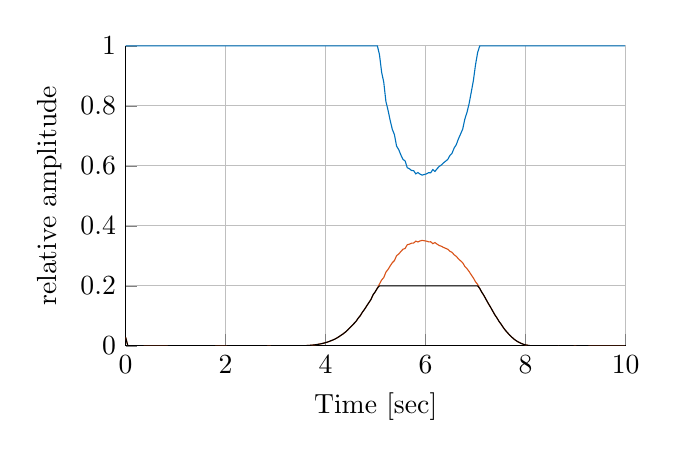
\begin{tikzpicture}

\begin{axis}[%
width=2.5in,
height=1.5in,
at={(0.758in,0.481in)},
scale only axis,
xmin=0,
xmax=10,
xlabel={Time [sec]},
xmajorgrids,
ymin=0,
ymax=1,
ylabel={relative amplitude},
ymajorgrids,
axis background/.style={fill=white},
axis x line*=bottom,
axis y line*=left
]
\addplot [color=mycolor1,solid,forget plot]
  table[row sep=crcr]{%
0	1\\
0.0426666666666667	1\\
0.0853333333333333	1\\
0.128	1\\
0.170666666666667	1\\
0.213333333333333	1\\
0.256	1\\
0.298666666666667	1\\
0.341333333333333	1\\
0.384	1\\
0.426666666666667	1\\
0.469333333333333	1\\
0.512	1\\
0.554666666666667	1\\
0.597333333333333	1\\
0.64	1\\
0.682666666666667	1\\
0.725333333333333	1\\
0.768	1\\
0.810666666666667	1\\
0.853333333333333	1\\
0.896	1\\
0.938666666666667	1\\
0.981333333333333	1\\
1.024	1\\
1.06666666666667	1\\
1.10933333333333	1\\
1.152	1\\
1.19466666666667	1\\
1.23733333333333	1\\
1.28	1\\
1.32266666666667	1\\
1.36533333333333	1\\
1.408	1\\
1.45066666666667	1\\
1.49333333333333	1\\
1.536	1\\
1.57866666666667	1\\
1.62133333333333	1\\
1.664	1\\
1.70666666666667	1\\
1.74933333333333	1\\
1.792	1\\
1.83466666666667	1\\
1.87733333333333	1\\
1.92	1\\
1.96266666666667	1\\
2.00533333333333	1\\
2.048	1\\
2.09066666666667	1\\
2.13333333333333	1\\
2.176	1\\
2.21866666666667	1\\
2.26133333333333	1\\
2.304	1\\
2.34666666666667	1\\
2.38933333333333	1\\
2.432	1\\
2.47466666666667	1\\
2.51733333333333	1\\
2.56	1\\
2.60266666666667	1\\
2.64533333333333	1\\
2.688	1\\
2.73066666666667	1\\
2.77333333333333	1\\
2.816	1\\
2.85866666666667	1\\
2.90133333333333	1\\
2.944	1\\
2.98666666666667	1\\
3.02933333333333	1\\
3.072	1\\
3.11466666666667	1\\
3.15733333333333	1\\
3.2	1\\
3.24266666666667	1\\
3.28533333333333	1\\
3.328	1\\
3.37066666666667	1\\
3.41333333333333	1\\
3.456	1\\
3.49866666666667	1\\
3.54133333333333	1\\
3.584	1\\
3.62666666666667	1\\
3.66933333333333	1\\
3.712	1\\
3.75466666666667	1\\
3.79733333333333	1\\
3.84	1\\
3.88266666666667	1\\
3.92533333333333	1\\
3.968	1\\
4.01066666666667	1\\
4.05333333333333	1\\
4.096	1\\
4.13866666666667	1\\
4.18133333333333	1\\
4.224	1\\
4.26666666666667	1\\
4.30933333333333	1\\
4.352	1\\
4.39466666666667	1\\
4.43733333333333	1\\
4.48	1\\
4.52266666666667	1\\
4.56533333333333	1\\
4.608	1\\
4.65066666666667	1\\
4.69333333333333	1\\
4.736	1\\
4.77866666666667	1\\
4.82133333333333	1\\
4.864	1\\
4.90666666666667	1\\
4.94933333333333	1\\
4.992	1\\
5.03466666666667	1\\
5.07733333333333	0.969880895980676\\
5.12	0.911709109696262\\
5.16266666666667	0.878566467045722\\
5.20533333333333	0.814684493807506\\
5.248	0.785362677451813\\
5.29066666666667	0.751385749497003\\
5.33333333333333	0.721769712703029\\
5.376	0.703640095623825\\
5.41866666666667	0.665847928629747\\
5.46133333333333	0.653946895360279\\
5.504	0.636420973537659\\
5.54666666666667	0.62121444677337\\
5.58933333333333	0.616347616719769\\
5.632	0.593789349850404\\
5.67466666666667	0.590311243223664\\
5.71733333333333	0.584503563699738\\
5.76	0.583871006663183\\
5.80266666666667	0.573174411309484\\
5.84533333333333	0.57762560767088\\
5.888	0.57223745755078\\
5.93066666666667	0.569074867692195\\
5.97333333333333	0.57105948822274\\
6.016	0.573066329461291\\
6.05866666666667	0.577110692498977\\
6.10133333333333	0.576760788197133\\
6.144	0.587394551662804\\
6.18666666666667	0.581267747476056\\
6.22933333333333	0.590269236135185\\
6.272	0.5982441738293\\
6.31466666666667	0.602738125651154\\
6.35733333333333	0.609779080921584\\
6.4	0.615461509713572\\
6.44266666666667	0.621351925592731\\
6.48533333333333	0.634259959142679\\
6.528	0.641876946247208\\
6.57066666666667	0.659518915310653\\
6.61333333333333	0.670547977484076\\
6.656	0.690059430798031\\
6.69866666666667	0.705887652442372\\
6.74133333333333	0.722388896704544\\
6.784	0.755932365552911\\
6.82666666666667	0.777977236375048\\
6.86933333333333	0.807285608013932\\
6.912	0.84520528220781\\
6.95466666666667	0.883876215146974\\
6.99733333333333	0.936482506162066\\
7.04	0.977712900587785\\
7.08266666666667	1\\
7.12533333333333	1\\
7.168	1\\
7.21066666666667	1\\
7.25333333333333	1\\
7.296	1\\
7.33866666666667	1\\
7.38133333333333	1\\
7.424	1\\
7.46666666666667	1\\
7.50933333333333	1\\
7.552	1\\
7.59466666666667	1\\
7.63733333333333	1\\
7.68	1\\
7.72266666666667	1\\
7.76533333333333	1\\
7.808	1\\
7.85066666666667	1\\
7.89333333333333	1\\
7.936	1\\
7.97866666666667	1\\
8.02133333333333	1\\
8.064	1\\
8.10666666666667	1\\
8.14933333333333	1\\
8.192	1\\
8.23466666666667	1\\
8.27733333333333	1\\
8.32	1\\
8.36266666666667	1\\
8.40533333333333	1\\
8.448	1\\
8.49066666666667	1\\
8.53333333333333	1\\
8.576	1\\
8.61866666666667	1\\
8.66133333333333	1\\
8.704	1\\
8.74666666666667	1\\
8.78933333333333	1\\
8.832	1\\
8.87466666666667	1\\
8.91733333333333	1\\
8.96	1\\
9.00266666666667	1\\
9.04533333333333	1\\
9.088	1\\
9.13066666666667	1\\
9.17333333333333	1\\
9.216	1\\
9.25866666666667	1\\
9.30133333333333	1\\
9.344	1\\
9.38666666666667	1\\
9.42933333333333	1\\
9.472	1\\
9.51466666666667	1\\
9.55733333333333	1\\
9.6	1\\
9.64266666666667	1\\
9.68533333333333	1\\
9.728	1\\
9.77066666666667	1\\
9.81333333333333	1\\
9.856	1\\
9.89866666666667	1\\
9.94133333333333	1\\
9.984	1\\
};
\addplot [color=mycolor2,solid,forget plot]
  table[row sep=crcr]{%
0	0.0282388040914952\\
0.0426666666666667	0.00107177953713978\\
0.0853333333333333	6.28322277133213e-05\\
0.128	6.49665856522593e-05\\
0.170666666666667	5.83868464472985e-05\\
0.213333333333333	5.08043003298312e-05\\
0.256	4.8447819329928e-05\\
0.298666666666667	4.44035819191288e-05\\
0.341333333333333	3.80201251988048e-05\\
0.384	3.15835569119565e-05\\
0.426666666666667	2.5695117576987e-05\\
0.469333333333333	1.99291890458e-05\\
0.512	1.39791291213467e-05\\
0.554666666666667	7.82340422532203e-06\\
0.597333333333333	2.20267674432613e-06\\
0.64	5.60656592377416e-06\\
0.682666666666667	1.14465812196147e-05\\
0.725333333333333	1.75207609088655e-05\\
0.768	2.50073515752096e-05\\
0.810666666666667	3.15048709393531e-05\\
0.853333333333333	3.53812050205405e-05\\
0.896	4.44403352882454e-05\\
0.938666666666667	4.80572456386141e-05\\
0.981333333333333	5.49958930516467e-05\\
1.024	5.8693480592249e-05\\
1.06666666666667	6.65131238276677e-05\\
1.10933333333333	6.61668485200097e-05\\
1.152	7.4041098114331e-05\\
1.19466666666667	7.80128851625685e-05\\
1.23733333333333	7.79403771648501e-05\\
1.28	7.94514346383498e-05\\
1.32266666666667	8.16230669727775e-05\\
1.36533333333333	8.26930397306177e-05\\
1.408	8.25229662096235e-05\\
1.45066666666667	8.15572060212458e-05\\
1.49333333333333	8.00416880344101e-05\\
1.536	7.71229284329365e-05\\
1.57866666666667	7.10465500759938e-05\\
1.62133333333333	6.43786247550614e-05\\
1.664	6.14024124341161e-05\\
1.70666666666667	5.22368110766006e-05\\
1.74933333333333	4.37160267878224e-05\\
1.792	3.47885808489743e-05\\
1.83466666666667	2.43032850853508e-05\\
1.87733333333333	1.26683506611189e-05\\
1.92	4.1347904167323e-06\\
1.96266666666667	1.38811607553244e-05\\
2.00533333333333	2.70409226730704e-05\\
2.048	4.07477350060181e-05\\
2.09066666666667	5.51389976683688e-05\\
2.13333333333333	6.98742071387533e-05\\
2.176	8.39647245982223e-05\\
2.21866666666667	9.57893935574026e-05\\
2.26133333333333	0.000108008190704394\\
2.304	0.000124763982117828\\
2.34666666666667	0.000129926160047441\\
2.38933333333333	0.000142138694949415\\
2.432	0.000144383738049175\\
2.47466666666667	0.000154316188525305\\
2.51733333333333	0.000149807323013747\\
2.56	0.000146600138013003\\
2.60266666666667	0.000142080808307791\\
2.64533333333333	0.000132051652374333\\
2.688	0.000117196748859266\\
2.73066666666667	9.82715692625955e-05\\
2.77333333333333	7.39593894762916e-05\\
2.816	4.34154052307768e-05\\
2.85866666666667	1.53033162143408e-05\\
2.90133333333333	3.33900286447377e-05\\
2.944	7.19208638780501e-05\\
2.98666666666667	0.000117360017831419\\
3.02933333333333	0.000167502865755585\\
3.072	0.00021345172886878\\
3.11466666666667	0.000258489780014376\\
3.15733333333333	0.000301001091552116\\
3.2	0.000334583831176306\\
3.24266666666667	0.00035377318834095\\
3.28533333333333	0.000370780497753704\\
3.328	0.000362265970105241\\
3.37066666666667	0.000321808686669682\\
3.41333333333333	0.000257397854317076\\
3.456	0.000163432124308274\\
3.49866666666667	0.00010493639872278\\
3.54133333333333	0.00027837531450186\\
3.584	0.000569112006237081\\
3.62666666666667	0.00094179447150661\\
3.66933333333333	0.00139524665768068\\
3.712	0.00205280604485173\\
3.75466666666667	0.00270005842820592\\
3.79733333333333	0.00369313134035538\\
3.84	0.00471216072352423\\
3.88266666666667	0.00593604378290063\\
3.92533333333333	0.00744733009468972\\
3.968	0.00921865529945331\\
4.01066666666667	0.0110687949817519\\
4.05333333333333	0.0133425132124141\\
4.096	0.0161953321181614\\
4.13866666666667	0.019068251958538\\
4.18133333333333	0.0221536157989619\\
4.224	0.0260460561497728\\
4.26666666666667	0.0303783140689522\\
4.30933333333333	0.0353854672964277\\
4.352	0.040129705882825\\
4.39466666666667	0.0456700149383858\\
4.43733333333333	0.0519624846596325\\
4.48	0.0594291720956924\\
4.52266666666667	0.0663835854317335\\
4.56533333333333	0.0739714738832096\\
4.608	0.0816703690843484\\
4.65066666666667	0.092165494523071\\
4.69333333333333	0.10053368445218\\
4.736	0.112392639964266\\
4.77866666666667	0.12185934165038\\
4.82133333333333	0.133037567077694\\
4.864	0.143898535505801\\
4.90666666666667	0.154518592404813\\
4.94933333333333	0.170258741912115\\
4.992	0.18007163495179\\
5.03466666666667	0.192233681808087\\
5.07733333333333	0.206210887160298\\
5.12	0.21936821500734\\
5.16266666666667	0.227643561986292\\
5.20533333333333	0.245493809591589\\
5.248	0.254659414996546\\
5.29066666666667	0.266174864420686\\
5.33333333333333	0.277096692310626\\
5.376	0.284236218549607\\
5.41866666666667	0.300368885147066\\
5.46133333333333	0.305835231299346\\
5.504	0.314257399293842\\
5.54666666666667	0.3219500142645\\
5.58933333333333	0.324492209549555\\
5.632	0.336819783060082\\
5.67466666666667	0.338804321103235\\
5.71733333333333	0.342170711045897\\
5.76	0.342541413630038\\
5.80266666666667	0.348933930150644\\
5.84533333333333	0.34624503717286\\
5.888	0.349505257583128\\
5.93066666666667	0.351447606201751\\
5.97333333333333	0.350226209571341\\
6.016	0.34899974002662\\
6.05866666666667	0.34655396720163\\
6.10133333333333	0.346764211598312\\
6.144	0.340486644681735\\
6.18666666666667	0.344075515747136\\
6.22933333333333	0.338828432444674\\
6.272	0.33431165525578\\
6.31466666666667	0.331819062854095\\
6.35733333333333	0.327987637256647\\
6.4	0.324959395256216\\
6.44266666666667	0.321878780385548\\
6.48533333333333	0.31532811919948\\
6.528	0.311586202260913\\
6.57066666666667	0.303251347849203\\
6.61333333333333	0.298263519860888\\
6.656	0.289830108935265\\
6.69866666666667	0.283331206188407\\
6.74133333333333	0.276859183346224\\
6.784	0.264573934274813\\
6.82666666666667	0.2570769305949\\
6.86933333333333	0.247743794779193\\
6.912	0.236628904492372\\
6.95466666666667	0.226276028897037\\
6.99733333333333	0.213565121274554\\
7.04	0.204559027378859\\
7.08266666666667	0.190986141168696\\
7.12533333333333	0.177952965165217\\
7.168	0.167052723635734\\
7.21066666666667	0.153853650034617\\
7.25333333333333	0.14119957383787\\
7.296	0.129314946925276\\
7.33866666666667	0.116792180043506\\
7.38133333333333	0.104022796329725\\
7.424	0.0935720561119066\\
7.46666666666667	0.0817486653016014\\
7.50933333333333	0.0719462298941643\\
7.552	0.0613382177620069\\
7.59466666666667	0.0517093229525832\\
7.63733333333333	0.0437403911100275\\
7.68	0.0356634185925986\\
7.72266666666667	0.0290396483683797\\
7.76533333333333	0.0226625954420665\\
7.808	0.0173429881341511\\
7.85066666666667	0.0129737136653792\\
7.89333333333333	0.00933552195306145\\
7.936	0.00626687344467878\\
7.97866666666667	0.00401320845815973\\
8.02133333333333	0.00227144925075129\\
8.064	0.00109583422209982\\
8.10666666666667	0.000336848341113091\\
8.14933333333333	0.000208654209436348\\
8.192	0.000358722364832184\\
8.23466666666667	0.00036549952567879\\
8.27733333333333	0.000271047729289022\\
8.32	0.000126254108709634\\
8.36266666666667	5.32340484034458e-05\\
8.40533333333333	0.000159649302908678\\
8.448	0.000232921522390117\\
8.49066666666667	0.000260046192551051\\
8.53333333333333	0.000234648305506217\\
8.576	0.000177093136625545\\
8.61866666666667	9.47816288826688e-05\\
8.66133333333333	2.49057269214853e-05\\
8.704	7.68591810786823e-05\\
8.74666666666667	0.00013233902313696\\
8.78933333333333	0.00015890345262837\\
8.832	0.000156857430637336\\
8.87466666666667	0.000129353824636095\\
8.91733333333333	8.52921055010737e-05\\
8.96	3.43793428498935e-05\\
9.00266666666667	2.4889489579921e-05\\
9.04533333333333	6.17941486169677e-05\\
9.088	8.37425720058614e-05\\
9.13066666666667	9.0693920244702e-05\\
9.17333333333333	7.96989621737035e-05\\
9.216	5.89861727917862e-05\\
9.25866666666667	3.17558913632554e-05\\
9.30133333333333	8.83733243099352e-06\\
9.344	1.51632412940633e-05\\
9.38666666666667	2.46696918983858e-05\\
9.42933333333333	2.58749399363198e-05\\
9.472	2.01244793422252e-05\\
9.51466666666667	1.00209650363962e-05\\
9.55733333333333	3.13749655473897e-06\\
9.6	9.32927812226036e-06\\
9.64266666666667	1.30573615888476e-05\\
9.68533333333333	1.28916380400308e-05\\
9.728	1.02917884950535e-05\\
9.77066666666667	5.75639553993091e-06\\
9.81333333333333	1.77821806118978e-06\\
9.856	1.39707160523351e-06\\
9.89866666666667	2.12896345007753e-06\\
9.94133333333333	2.00120638913694e-06\\
9.984	1.37552429553707e-05\\
};
\addplot [color=mycolor3,solid,forget plot]
  table[row sep=crcr]{%
0	0.0282388040914952\\
0.0426666666666667	0.00107177953713978\\
0.0853333333333333	6.28322277133213e-05\\
0.128	6.49665856522593e-05\\
0.170666666666667	5.83868464472985e-05\\
0.213333333333333	5.08043003298312e-05\\
0.256	4.8447819329928e-05\\
0.298666666666667	4.44035819191288e-05\\
0.341333333333333	3.80201251988048e-05\\
0.384	3.15835569119565e-05\\
0.426666666666667	2.5695117576987e-05\\
0.469333333333333	1.99291890458e-05\\
0.512	1.39791291213467e-05\\
0.554666666666667	7.82340422532203e-06\\
0.597333333333333	2.20267674432613e-06\\
0.64	5.60656592377416e-06\\
0.682666666666667	1.14465812196147e-05\\
0.725333333333333	1.75207609088655e-05\\
0.768	2.50073515752096e-05\\
0.810666666666667	3.15048709393531e-05\\
0.853333333333333	3.53812050205405e-05\\
0.896	4.44403352882454e-05\\
0.938666666666667	4.80572456386141e-05\\
0.981333333333333	5.49958930516467e-05\\
1.024	5.8693480592249e-05\\
1.06666666666667	6.65131238276677e-05\\
1.10933333333333	6.61668485200097e-05\\
1.152	7.4041098114331e-05\\
1.19466666666667	7.80128851625685e-05\\
1.23733333333333	7.79403771648501e-05\\
1.28	7.94514346383498e-05\\
1.32266666666667	8.16230669727775e-05\\
1.36533333333333	8.26930397306177e-05\\
1.408	8.25229662096235e-05\\
1.45066666666667	8.15572060212458e-05\\
1.49333333333333	8.00416880344101e-05\\
1.536	7.71229284329365e-05\\
1.57866666666667	7.10465500759938e-05\\
1.62133333333333	6.43786247550614e-05\\
1.664	6.14024124341161e-05\\
1.70666666666667	5.22368110766006e-05\\
1.74933333333333	4.37160267878224e-05\\
1.792	3.47885808489743e-05\\
1.83466666666667	2.43032850853508e-05\\
1.87733333333333	1.26683506611189e-05\\
1.92	4.1347904167323e-06\\
1.96266666666667	1.38811607553244e-05\\
2.00533333333333	2.70409226730704e-05\\
2.048	4.07477350060181e-05\\
2.09066666666667	5.51389976683688e-05\\
2.13333333333333	6.98742071387533e-05\\
2.176	8.39647245982223e-05\\
2.21866666666667	9.57893935574026e-05\\
2.26133333333333	0.000108008190704394\\
2.304	0.000124763982117828\\
2.34666666666667	0.000129926160047441\\
2.38933333333333	0.000142138694949415\\
2.432	0.000144383738049175\\
2.47466666666667	0.000154316188525305\\
2.51733333333333	0.000149807323013747\\
2.56	0.000146600138013003\\
2.60266666666667	0.000142080808307791\\
2.64533333333333	0.000132051652374333\\
2.688	0.000117196748859266\\
2.73066666666667	9.82715692625955e-05\\
2.77333333333333	7.39593894762916e-05\\
2.816	4.34154052307768e-05\\
2.85866666666667	1.53033162143408e-05\\
2.90133333333333	3.33900286447377e-05\\
2.944	7.19208638780501e-05\\
2.98666666666667	0.000117360017831419\\
3.02933333333333	0.000167502865755585\\
3.072	0.00021345172886878\\
3.11466666666667	0.000258489780014376\\
3.15733333333333	0.000301001091552116\\
3.2	0.000334583831176306\\
3.24266666666667	0.00035377318834095\\
3.28533333333333	0.000370780497753704\\
3.328	0.000362265970105241\\
3.37066666666667	0.000321808686669682\\
3.41333333333333	0.000257397854317076\\
3.456	0.000163432124308274\\
3.49866666666667	0.00010493639872278\\
3.54133333333333	0.00027837531450186\\
3.584	0.000569112006237081\\
3.62666666666667	0.00094179447150661\\
3.66933333333333	0.00139524665768068\\
3.712	0.00205280604485173\\
3.75466666666667	0.00270005842820592\\
3.79733333333333	0.00369313134035538\\
3.84	0.00471216072352423\\
3.88266666666667	0.00593604378290063\\
3.92533333333333	0.00744733009468972\\
3.968	0.00921865529945331\\
4.01066666666667	0.0110687949817519\\
4.05333333333333	0.0133425132124141\\
4.096	0.0161953321181614\\
4.13866666666667	0.019068251958538\\
4.18133333333333	0.0221536157989619\\
4.224	0.0260460561497728\\
4.26666666666667	0.0303783140689522\\
4.30933333333333	0.0353854672964277\\
4.352	0.040129705882825\\
4.39466666666667	0.0456700149383858\\
4.43733333333333	0.0519624846596325\\
4.48	0.0594291720956924\\
4.52266666666667	0.0663835854317335\\
4.56533333333333	0.0739714738832096\\
4.608	0.0816703690843484\\
4.65066666666667	0.092165494523071\\
4.69333333333333	0.10053368445218\\
4.736	0.112392639964266\\
4.77866666666667	0.12185934165038\\
4.82133333333333	0.133037567077694\\
4.864	0.143898535505801\\
4.90666666666667	0.154518592404813\\
4.94933333333333	0.170258741912115\\
4.992	0.18007163495179\\
5.03466666666667	0.192233681808087\\
5.07733333333333	0.2\\
5.12	0.2\\
5.16266666666667	0.2\\
5.20533333333333	0.2\\
5.248	0.2\\
5.29066666666667	0.2\\
5.33333333333333	0.2\\
5.376	0.2\\
5.41866666666667	0.2\\
5.46133333333333	0.2\\
5.504	0.2\\
5.54666666666667	0.2\\
5.58933333333333	0.2\\
5.632	0.2\\
5.67466666666667	0.2\\
5.71733333333333	0.2\\
5.76	0.2\\
5.80266666666667	0.2\\
5.84533333333333	0.2\\
5.888	0.2\\
5.93066666666667	0.2\\
5.97333333333333	0.2\\
6.016	0.2\\
6.05866666666667	0.2\\
6.10133333333333	0.2\\
6.144	0.2\\
6.18666666666667	0.2\\
6.22933333333333	0.2\\
6.272	0.2\\
6.31466666666667	0.2\\
6.35733333333333	0.2\\
6.4	0.2\\
6.44266666666667	0.2\\
6.48533333333333	0.2\\
6.528	0.2\\
6.57066666666667	0.2\\
6.61333333333333	0.2\\
6.656	0.2\\
6.69866666666667	0.2\\
6.74133333333333	0.2\\
6.784	0.2\\
6.82666666666667	0.2\\
6.86933333333333	0.2\\
6.912	0.2\\
6.95466666666667	0.2\\
6.99733333333333	0.2\\
7.04	0.2\\
7.08266666666667	0.190986141168696\\
7.12533333333333	0.177952965165217\\
7.168	0.167052723635734\\
7.21066666666667	0.153853650034617\\
7.25333333333333	0.14119957383787\\
7.296	0.129314946925276\\
7.33866666666667	0.116792180043506\\
7.38133333333333	0.104022796329725\\
7.424	0.0935720561119066\\
7.46666666666667	0.0817486653016014\\
7.50933333333333	0.0719462298941643\\
7.552	0.0613382177620069\\
7.59466666666667	0.0517093229525832\\
7.63733333333333	0.0437403911100275\\
7.68	0.0356634185925986\\
7.72266666666667	0.0290396483683797\\
7.76533333333333	0.0226625954420665\\
7.808	0.0173429881341511\\
7.85066666666667	0.0129737136653792\\
7.89333333333333	0.00933552195306145\\
7.936	0.00626687344467878\\
7.97866666666667	0.00401320845815973\\
8.02133333333333	0.00227144925075129\\
8.064	0.00109583422209982\\
8.10666666666667	0.000336848341113091\\
8.14933333333333	0.000208654209436348\\
8.192	0.000358722364832184\\
8.23466666666667	0.00036549952567879\\
8.27733333333333	0.000271047729289022\\
8.32	0.000126254108709634\\
8.36266666666667	5.32340484034458e-05\\
8.40533333333333	0.000159649302908678\\
8.448	0.000232921522390117\\
8.49066666666667	0.000260046192551051\\
8.53333333333333	0.000234648305506217\\
8.576	0.000177093136625545\\
8.61866666666667	9.47816288826688e-05\\
8.66133333333333	2.49057269214853e-05\\
8.704	7.68591810786823e-05\\
8.74666666666667	0.00013233902313696\\
8.78933333333333	0.00015890345262837\\
8.832	0.000156857430637336\\
8.87466666666667	0.000129353824636095\\
8.91733333333333	8.52921055010737e-05\\
8.96	3.43793428498935e-05\\
9.00266666666667	2.4889489579921e-05\\
9.04533333333333	6.17941486169677e-05\\
9.088	8.37425720058614e-05\\
9.13066666666667	9.0693920244702e-05\\
9.17333333333333	7.96989621737035e-05\\
9.216	5.89861727917862e-05\\
9.25866666666667	3.17558913632554e-05\\
9.30133333333333	8.83733243099352e-06\\
9.344	1.51632412940633e-05\\
9.38666666666667	2.46696918983858e-05\\
9.42933333333333	2.58749399363198e-05\\
9.472	2.01244793422252e-05\\
9.51466666666667	1.00209650363962e-05\\
9.55733333333333	3.13749655473897e-06\\
9.6	9.32927812226036e-06\\
9.64266666666667	1.30573615888476e-05\\
9.68533333333333	1.28916380400308e-05\\
9.728	1.02917884950535e-05\\
9.77066666666667	5.75639553993091e-06\\
9.81333333333333	1.77821806118978e-06\\
9.856	1.39707160523351e-06\\
9.89866666666667	2.12896345007753e-06\\
9.94133333333333	2.00120638913694e-06\\
9.984	1.37552429553707e-05\\
};
\end{axis}
\end{tikzpicture}%
    \caption{Band 3 from 132 Hz to 265 Hz}
    \label{fig:Band3Simulation}
\end{subfigure}
\begin{subfigure}[t]{0.49\textwidth}
    \centering
    \tikzsetnextfilename{Band4Simulation}
    % This file was created by matlab2tikz.
%
%The latest updates can be retrieved from
%  http://www.mathworks.com/matlabcentral/fileexchange/22022-matlab2tikz-matlab2tikz
%where you can also make suggestions and rate matlab2tikz.
%
\definecolor{mycolor1}{rgb}{0.00000,0.44700,0.74100}%
\definecolor{mycolor2}{rgb}{0.85000,0.32500,0.09800}%
\definecolor{mycolor3}{rgb}{0.00,0.00,0.00}%
%
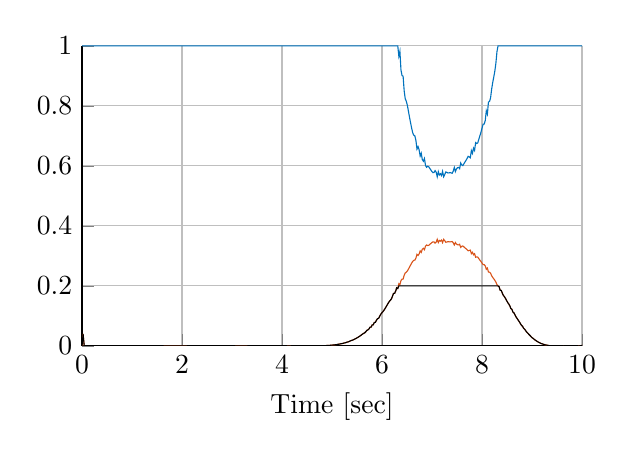
\begin{tikzpicture}

\begin{axis}[%
width=2.5in,
height=1.5in,
scale only axis,
xmin=0,
xmax=10,
xlabel={Time [sec]},
xmajorgrids,
ymin=0,
ymax=1,
ymajorgrids,
axis background/.style={fill=white},
axis x line*=bottom,
axis y line*=left
]
\addplot [color=mycolor1,solid,forget plot]
  table[row sep=crcr]{%
0	1\\
0.0213333333333333	1\\
0.0426666666666667	1\\
0.064	1\\
0.0853333333333333	1\\
0.106666666666667	1\\
0.128	1\\
0.149333333333333	1\\
0.170666666666667	1\\
0.192	1\\
0.213333333333333	1\\
0.234666666666667	1\\
0.256	1\\
0.277333333333333	1\\
0.298666666666667	1\\
0.32	1\\
0.341333333333333	1\\
0.362666666666667	1\\
0.384	1\\
0.405333333333333	1\\
0.426666666666667	1\\
0.448	1\\
0.469333333333333	1\\
0.490666666666667	1\\
0.512	1\\
0.533333333333333	1\\
0.554666666666667	1\\
0.576	1\\
0.597333333333333	1\\
0.618666666666667	1\\
0.64	1\\
0.661333333333333	1\\
0.682666666666667	1\\
0.704	1\\
0.725333333333333	1\\
0.746666666666667	1\\
0.768	1\\
0.789333333333333	1\\
0.810666666666667	1\\
0.832	1\\
0.853333333333333	1\\
0.874666666666667	1\\
0.896	1\\
0.917333333333333	1\\
0.938666666666667	1\\
0.96	1\\
0.981333333333333	1\\
1.00266666666667	1\\
1.024	1\\
1.04533333333333	1\\
1.06666666666667	1\\
1.088	1\\
1.10933333333333	1\\
1.13066666666667	1\\
1.152	1\\
1.17333333333333	1\\
1.19466666666667	1\\
1.216	1\\
1.23733333333333	1\\
1.25866666666667	1\\
1.28	1\\
1.30133333333333	1\\
1.32266666666667	1\\
1.344	1\\
1.36533333333333	1\\
1.38666666666667	1\\
1.408	1\\
1.42933333333333	1\\
1.45066666666667	1\\
1.472	1\\
1.49333333333333	1\\
1.51466666666667	1\\
1.536	1\\
1.55733333333333	1\\
1.57866666666667	1\\
1.6	1\\
1.62133333333333	1\\
1.64266666666667	1\\
1.664	1\\
1.68533333333333	1\\
1.70666666666667	1\\
1.728	1\\
1.74933333333333	1\\
1.77066666666667	1\\
1.792	1\\
1.81333333333333	1\\
1.83466666666667	1\\
1.856	1\\
1.87733333333333	1\\
1.89866666666667	1\\
1.92	1\\
1.94133333333333	1\\
1.96266666666667	1\\
1.984	1\\
2.00533333333333	1\\
2.02666666666667	1\\
2.048	1\\
2.06933333333333	1\\
2.09066666666667	1\\
2.112	1\\
2.13333333333333	1\\
2.15466666666667	1\\
2.176	1\\
2.19733333333333	1\\
2.21866666666667	1\\
2.24	1\\
2.26133333333333	1\\
2.28266666666667	1\\
2.304	1\\
2.32533333333333	1\\
2.34666666666667	1\\
2.368	1\\
2.38933333333333	1\\
2.41066666666667	1\\
2.432	1\\
2.45333333333333	1\\
2.47466666666667	1\\
2.496	1\\
2.51733333333333	1\\
2.53866666666667	1\\
2.56	1\\
2.58133333333333	1\\
2.60266666666667	1\\
2.624	1\\
2.64533333333333	1\\
2.66666666666667	1\\
2.688	1\\
2.70933333333333	1\\
2.73066666666667	1\\
2.752	1\\
2.77333333333333	1\\
2.79466666666667	1\\
2.816	1\\
2.83733333333333	1\\
2.85866666666667	1\\
2.88	1\\
2.90133333333333	1\\
2.92266666666667	1\\
2.944	1\\
2.96533333333333	1\\
2.98666666666667	1\\
3.008	1\\
3.02933333333333	1\\
3.05066666666667	1\\
3.072	1\\
3.09333333333333	1\\
3.11466666666667	1\\
3.136	1\\
3.15733333333333	1\\
3.17866666666667	1\\
3.2	1\\
3.22133333333333	1\\
3.24266666666667	1\\
3.264	1\\
3.28533333333333	1\\
3.30666666666667	1\\
3.328	1\\
3.34933333333333	1\\
3.37066666666667	1\\
3.392	1\\
3.41333333333333	1\\
3.43466666666667	1\\
3.456	1\\
3.47733333333333	1\\
3.49866666666667	1\\
3.52	1\\
3.54133333333333	1\\
3.56266666666667	1\\
3.584	1\\
3.60533333333333	1\\
3.62666666666667	1\\
3.648	1\\
3.66933333333333	1\\
3.69066666666667	1\\
3.712	1\\
3.73333333333333	1\\
3.75466666666667	1\\
3.776	1\\
3.79733333333333	1\\
3.81866666666667	1\\
3.84	1\\
3.86133333333333	1\\
3.88266666666667	1\\
3.904	1\\
3.92533333333333	1\\
3.94666666666667	1\\
3.968	1\\
3.98933333333333	1\\
4.01066666666667	1\\
4.032	1\\
4.05333333333333	1\\
4.07466666666667	1\\
4.096	1\\
4.11733333333333	1\\
4.13866666666667	1\\
4.16	1\\
4.18133333333333	1\\
4.20266666666667	1\\
4.224	1\\
4.24533333333333	1\\
4.26666666666667	1\\
4.288	1\\
4.30933333333333	1\\
4.33066666666667	1\\
4.352	1\\
4.37333333333333	1\\
4.39466666666667	1\\
4.416	1\\
4.43733333333333	1\\
4.45866666666667	1\\
4.48	1\\
4.50133333333333	1\\
4.52266666666667	1\\
4.544	1\\
4.56533333333333	1\\
4.58666666666667	1\\
4.608	1\\
4.62933333333333	1\\
4.65066666666667	1\\
4.672	1\\
4.69333333333333	1\\
4.71466666666667	1\\
4.736	1\\
4.75733333333333	1\\
4.77866666666667	1\\
4.8	1\\
4.82133333333333	1\\
4.84266666666667	1\\
4.864	1\\
4.88533333333333	1\\
4.90666666666667	1\\
4.928	1\\
4.94933333333333	1\\
4.97066666666667	1\\
4.992	1\\
5.01333333333333	1\\
5.03466666666667	1\\
5.056	1\\
5.07733333333333	1\\
5.09866666666667	1\\
5.12	1\\
5.14133333333333	1\\
5.16266666666667	1\\
5.184	1\\
5.20533333333333	1\\
5.22666666666667	1\\
5.248	1\\
5.26933333333333	1\\
5.29066666666667	1\\
5.312	1\\
5.33333333333333	1\\
5.35466666666667	1\\
5.376	1\\
5.39733333333333	1\\
5.41866666666667	1\\
5.44	1\\
5.46133333333333	1\\
5.48266666666667	1\\
5.504	1\\
5.52533333333333	1\\
5.54666666666667	1\\
5.568	1\\
5.58933333333333	1\\
5.61066666666667	1\\
5.632	1\\
5.65333333333333	1\\
5.67466666666667	1\\
5.696	1\\
5.71733333333333	1\\
5.73866666666667	1\\
5.76	1\\
5.78133333333333	1\\
5.80266666666667	1\\
5.824	1\\
5.84533333333333	1\\
5.86666666666667	1\\
5.888	1\\
5.90933333333333	1\\
5.93066666666667	1\\
5.952	1\\
5.97333333333333	1\\
5.99466666666667	1\\
6.016	1\\
6.03733333333333	1\\
6.05866666666667	1\\
6.08	1\\
6.10133333333333	1\\
6.12266666666667	1\\
6.144	1\\
6.16533333333333	1\\
6.18666666666667	1\\
6.208	1\\
6.22933333333333	1\\
6.25066666666667	1\\
6.272	1\\
6.29333333333333	1\\
6.31466666666667	1\\
6.336	0.9653280437395\\
6.35733333333333	0.981858691701559\\
6.37866666666667	0.91941644163458\\
6.4	0.900681460784169\\
6.42133333333333	0.898791515558405\\
6.44266666666667	0.849899759421221\\
6.464	0.823466828178214\\
6.48533333333333	0.814990102889263\\
6.50666666666667	0.801401737714459\\
6.528	0.781898655354693\\
6.54933333333333	0.762035673074443\\
6.57066666666667	0.743444922836831\\
6.592	0.725762623848362\\
6.61333333333333	0.710324527048778\\
6.63466666666667	0.701821482058343\\
6.656	0.700143118159379\\
6.67733333333333	0.684694463086329\\
6.69866666666667	0.655721023390825\\
6.72	0.663982857197973\\
6.74133333333333	0.653396132877242\\
6.76266666666667	0.632353643910407\\
6.784	0.641871788612843\\
6.80533333333333	0.621055652727582\\
6.82666666666667	0.615203610291529\\
6.848	0.624359838472092\\
6.86933333333333	0.601440706166282\\
6.89066666666667	0.594923707024997\\
6.912	0.598446878431474\\
6.93333333333333	0.596963942981492\\
6.95466666666667	0.591669789515793\\
6.976	0.586097786894644\\
6.99733333333333	0.580973594956362\\
7.01866666666667	0.577098577427096\\
7.04	0.577950345109223\\
7.06133333333333	0.584154459481251\\
7.08266666666667	0.578884129941937\\
7.104	0.563453253884971\\
7.12533333333333	0.580610577630614\\
7.14666666666667	0.569549593877126\\
7.168	0.573403544520537\\
7.18933333333333	0.567457516937852\\
7.21066666666667	0.581341487907051\\
7.232	0.56343720103443\\
7.25333333333333	0.570667294761365\\
7.27466666666667	0.579518998452039\\
7.296	0.578146644718076\\
7.31733333333333	0.576138728455893\\
7.33866666666667	0.576494320159001\\
7.36	0.577317306954974\\
7.38133333333333	0.576407876521265\\
7.40266666666667	0.575100271969709\\
7.424	0.582360304990858\\
7.44533333333333	0.594572566280857\\
7.46666666666667	0.580796152940491\\
7.488	0.589560669749792\\
7.50933333333333	0.593694270961209\\
7.53066666666667	0.594547705941301\\
7.552	0.590681021423024\\
7.57333333333333	0.609341883117137\\
7.59466666666667	0.602832294971325\\
7.616	0.600689297846316\\
7.63733333333333	0.606647230143905\\
7.65866666666667	0.612752964002066\\
7.68	0.618157310886169\\
7.70133333333333	0.624905642473558\\
7.72266666666667	0.631624853207863\\
7.744	0.629455107492503\\
7.76533333333333	0.62682602127786\\
7.78666666666667	0.650713536282727\\
7.808	0.641548299846129\\
7.82933333333333	0.658752103819904\\
7.85066666666667	0.651374359617088\\
7.872	0.677356883981526\\
7.89333333333333	0.674331952133753\\
7.91466666666667	0.676572822248399\\
7.936	0.688529447928394\\
7.95733333333333	0.700348429198823\\
7.97866666666667	0.711778141061645\\
8	0.725607429193488\\
8.02133333333333	0.738578414632255\\
8.04266666666667	0.739059422110585\\
8.064	0.750476389060964\\
8.08533333333333	0.783395335415332\\
8.10666666666667	0.772163480874973\\
8.128	0.812611645482887\\
8.14933333333333	0.81439741579535\\
8.17066666666667	0.826305197077286\\
8.192	0.855487270058899\\
8.21333333333333	0.877473132452843\\
8.23466666666667	0.895902013853199\\
8.256	0.915848802269921\\
8.27733333333333	0.942447186238198\\
8.29866666666667	0.980703329880243\\
8.32	1\\
8.34133333333333	1\\
8.36266666666667	1\\
8.384	1\\
8.40533333333333	1\\
8.42666666666667	1\\
8.448	1\\
8.46933333333333	1\\
8.49066666666667	1\\
8.512	1\\
8.53333333333333	1\\
8.55466666666667	1\\
8.576	1\\
8.59733333333333	1\\
8.61866666666667	1\\
8.64	1\\
8.66133333333333	1\\
8.68266666666667	1\\
8.704	1\\
8.72533333333333	1\\
8.74666666666667	1\\
8.768	1\\
8.78933333333333	1\\
8.81066666666667	1\\
8.832	1\\
8.85333333333333	1\\
8.87466666666667	1\\
8.896	1\\
8.91733333333333	1\\
8.93866666666667	1\\
8.96	1\\
8.98133333333333	1\\
9.00266666666667	1\\
9.024	1\\
9.04533333333333	1\\
9.06666666666667	1\\
9.088	1\\
9.10933333333333	1\\
9.13066666666667	1\\
9.152	1\\
9.17333333333333	1\\
9.19466666666667	1\\
9.216	1\\
9.23733333333333	1\\
9.25866666666667	1\\
9.28	1\\
9.30133333333333	1\\
9.32266666666667	1\\
9.344	1\\
9.36533333333333	1\\
9.38666666666667	1\\
9.408	1\\
9.42933333333333	1\\
9.45066666666667	1\\
9.472	1\\
9.49333333333333	1\\
9.51466666666667	1\\
9.536	1\\
9.55733333333333	1\\
9.57866666666667	1\\
9.6	1\\
9.62133333333333	1\\
9.64266666666667	1\\
9.664	1\\
9.68533333333333	1\\
9.70666666666667	1\\
9.728	1\\
9.74933333333333	1\\
9.77066666666667	1\\
9.792	1\\
9.81333333333333	1\\
9.83466666666667	1\\
9.856	1\\
9.87733333333333	1\\
9.89866666666667	1\\
9.92	1\\
9.94133333333333	1\\
9.96266666666667	1\\
9.984	1\\
10.0053333333333	1\\
};
\addplot [color=mycolor2,solid,forget plot]
  table[row sep=crcr]{%
0	0.000393103114443459\\
0.0213333333333333	0.0393915477580857\\
0.0426666666666667	0.00146511568754698\\
0.064	8.36030774515732e-05\\
0.0853333333333333	8.11176679805252e-05\\
0.106666666666667	8.278439558703e-05\\
0.128	8.73031560982029e-05\\
0.149333333333333	9.20605803312465e-05\\
0.170666666666667	9.52132286331179e-05\\
0.192	9.62244620117345e-05\\
0.213333333333333	9.55244633907065e-05\\
0.234666666666667	9.39926501886425e-05\\
0.256	9.25093024211933e-05\\
0.277333333333333	9.16603167728589e-05\\
0.298666666666667	9.16375656339722e-05\\
0.32	9.23169504411538e-05\\
0.341333333333333	9.34228560874352e-05\\
0.362666666666667	9.46749570817113e-05\\
0.384	9.58670332112705e-05\\
0.405333333333333	9.6884054299269e-05\\
0.426666666666667	9.76855374666473e-05\\
0.448	9.82790996506004e-05\\
0.469333333333333	9.86972146230631e-05\\
0.490666666666667	9.89817041102552e-05\\
0.512	9.91758761027263e-05\\
0.533333333333333	9.93222876109235e-05\\
0.554666666666667	9.94635129899748e-05\\
0.576	9.96431393637136e-05\\
0.597333333333333	9.99040722080964e-05\\
0.618666666666667	0.000100281204120521\\
0.64	0.000100786196240015\\
0.661333333333333	0.000101384545315458\\
0.682666666666667	0.000101970049850335\\
0.704	0.000102348824979068\\
0.725333333333333	0.00010225185666109\\
0.746666666666667	0.000101398058319511\\
0.768	9.96243436949984e-05\\
0.789333333333333	9.70766495181219e-05\\
0.810666666666667	9.43947491643339e-05\\
0.832	9.26991757682527e-05\\
0.853333333333333	9.3089834867379e-05\\
0.874666666666667	9.56780955894731e-05\\
0.896	9.89691423306533e-05\\
0.917333333333333	0.000100440379927536\\
0.938666666666667	9.8086026869083e-05\\
0.96	9.22120976881714e-05\\
0.981333333333333	8.65984717109152e-05\\
1.00266666666667	8.64560109970826e-05\\
1.024	9.17980008154481e-05\\
1.04533333333333	9.57626792841925e-05\\
1.06666666666667	9.22193934937868e-05\\
1.088	8.30466389792519e-05\\
1.10933333333333	7.91453831259259e-05\\
1.13066666666667	8.55666987446584e-05\\
1.152	9.00280164239099e-05\\
1.17333333333333	8.27911710533397e-05\\
1.19466666666667	7.29106351831906e-05\\
1.216	7.71110124980109e-05\\
1.23733333333333	8.37377114602232e-05\\
1.25866666666667	7.57636062042899e-05\\
1.28	6.60968486245003e-05\\
1.30133333333333	7.36562121886799e-05\\
1.32266666666667	7.53250812879496e-05\\
1.344	6.22648910667071e-05\\
1.36533333333333	6.36419998379241e-05\\
1.38666666666667	6.97478535585958e-05\\
1.408	5.75873587725975e-05\\
1.42933333333333	5.66857685467256e-05\\
1.45066666666667	6.24549196666172e-05\\
1.472	4.98667079654651e-05\\
1.49333333333333	5.21984818929534e-05\\
1.51466666666667	5.3144772788039e-05\\
1.536	4.1662761052108e-05\\
1.55733333333333	4.82762895047967e-05\\
1.57866666666667	4.00983364645556e-05\\
1.6	3.83167174391871e-05\\
1.62133333333333	3.86750928014442e-05\\
1.64266666666667	3.0084186974945e-05\\
1.664	3.37936547599372e-05\\
1.68533333333333	2.45906302401587e-05\\
1.70666666666667	2.71196084186702e-05\\
1.728	1.97664884618302e-05\\
1.74933333333333	2.02201113910977e-05\\
1.77066666666667	1.4464616262668e-05\\
1.792	1.35313812303684e-05\\
1.81333333333333	8.70745294125698e-06\\
1.83466666666667	6.89139788271158e-06\\
1.856	2.90279823866731e-06\\
1.87733333333333	1.13681741605359e-06\\
1.89866666666667	3.10922290907567e-06\\
1.92	6.93697524934423e-06\\
1.94133333333333	9.66821947588814e-06\\
1.96266666666667	1.25219524024488e-05\\
1.984	1.74922476853785e-05\\
2.00533333333333	1.75673257576689e-05\\
2.02666666666667	2.3991607514697e-05\\
2.048	2.611476102035e-05\\
2.06933333333333	2.68303178782026e-05\\
2.09066666666667	3.46013125974599e-05\\
2.112	3.49293297387465e-05\\
2.13333333333333	3.57289192087958e-05\\
2.15466666666667	4.39623915087804e-05\\
2.176	4.53285970039883e-05\\
2.19733333333333	4.37659664245671e-05\\
2.21866666666667	5.05258601156612e-05\\
2.24	5.62984654075197e-05\\
2.26133333333333	5.49302090318167e-05\\
2.28266666666667	5.46626590083086e-05\\
2.304	6.08118808707166e-05\\
2.32533333333333	6.65339497003085e-05\\
2.34666666666667	6.72063877562728e-05\\
2.368	6.56799426857858e-05\\
2.38933333333333	6.67518415466299e-05\\
2.41066666666667	7.09749958100428e-05\\
2.432	7.54105409026009e-05\\
2.45333333333333	7.795697343936e-05\\
2.47466666666667	7.86028980963055e-05\\
2.496	7.84213269180532e-05\\
2.51733333333333	7.84102300929342e-05\\
2.53866666666667	7.89542534280644e-05\\
2.56	7.99142875864059e-05\\
2.58133333333333	8.09672784879229e-05\\
2.60266666666667	8.1851979869725e-05\\
2.624	8.24399069801979e-05\\
2.64533333333333	8.27075890073782e-05\\
2.66666666666667	8.26883900996913e-05\\
2.688	8.24369704517364e-05\\
2.70933333333333	8.2007151868556e-05\\
2.73066666666667	8.14310439911323e-05\\
2.752	8.06878500201144e-05\\
2.77333333333333	7.96639317899121e-05\\
2.79466666666667	7.81332525719662e-05\\
2.816	7.58200667608686e-05\\
2.83733333333333	7.26090052214623e-05\\
2.85866666666667	6.88740586032486e-05\\
2.88	6.56205165632365e-05\\
2.90133333333333	6.38127645569288e-05\\
2.92266666666667	6.29195890001885e-05\\
2.944	6.06448391085944e-05\\
2.96533333333333	5.52717323535829e-05\\
2.98666666666667	4.86260640617562e-05\\
3.008	4.49793062442906e-05\\
3.02933333333333	4.34572444792338e-05\\
3.05066666666667	3.84625024836987e-05\\
3.072	3.06908781218238e-05\\
3.09333333333333	2.64881524898199e-05\\
3.11466666666667	2.27605627755612e-05\\
3.136	1.53538444673849e-05\\
3.15733333333333	9.77466336133498e-06\\
3.17866666666667	4.60751853120477e-06\\
3.2	3.59875350152214e-06\\
3.22133333333333	9.04595293751445e-06\\
3.24266666666667	1.69368717446728e-05\\
3.264	2.12108725709466e-05\\
3.28533333333333	3.13815855117677e-05\\
3.30666666666667	3.47829935255419e-05\\
3.328	4.54756699481723e-05\\
3.34933333333333	4.90912036542668e-05\\
3.37066666666667	6.00533850572119e-05\\
3.392	6.25797280277317e-05\\
3.41333333333333	7.5858025203948e-05\\
3.43466666666667	7.47147683202184e-05\\
3.456	9.15283459675509e-05\\
3.47733333333333	8.87249529192109e-05\\
3.49866666666667	0.000101600211000484\\
3.52	0.000109197918788123\\
3.54133333333333	0.000106535258336914\\
3.56266666666667	0.00012290254228268\\
3.584	0.00012618493999033\\
3.60533333333333	0.000123090792131973\\
3.62666666666667	0.000135687639423944\\
3.648	0.000143925087761855\\
3.66933333333333	0.00014030048245714\\
3.69066666666667	0.000140167551143864\\
3.712	0.000148041611067319\\
3.73333333333333	0.000154261552783066\\
3.75466666666667	0.000154309881294435\\
3.776	0.000151159698548003\\
3.79733333333333	0.000148523728133556\\
3.81866666666667	0.000147230849638775\\
3.84	0.000146131809319259\\
3.86133333333333	0.000144048211090626\\
3.88266666666667	0.000140492227644624\\
3.904	0.000135469095740518\\
3.92533333333333	0.000129151670749856\\
3.94666666666667	0.000121712336363077\\
3.968	0.000113272820315045\\
3.98933333333333	0.00010386416327247\\
4.01066666666667	9.3337484889011e-05\\
4.032	8.12959851441534e-05\\
4.05333333333333	6.72927913818631e-05\\
4.07466666666667	5.14971182222586e-05\\
4.096	3.53329497713026e-05\\
4.11733333333333	2.04640272633392e-05\\
4.13866666666667	8.78560588892844e-06\\
4.16	2.06965660972415e-05\\
4.18133333333333	4.11213575308711e-05\\
4.20266666666667	5.84562062196122e-05\\
4.224	8.12677184302848e-05\\
4.24533333333333	0.000108963705082318\\
4.26666666666667	0.000123815063457753\\
4.288	0.000150886127623025\\
4.30933333333333	0.000180635235008118\\
4.33066666666667	0.000189723730847528\\
4.352	0.000232265395382198\\
4.37333333333333	0.000235412636322256\\
4.39466666666667	0.000277368777331768\\
4.416	0.000278256610113459\\
4.43733333333333	0.0003206140444055\\
4.45866666666667	0.000311727885297325\\
4.48	0.000355925921127085\\
4.50133333333333	0.000344440538646883\\
4.52266666666667	0.000362683183566128\\
4.544	0.000380552287566966\\
4.56533333333333	0.000357399288632821\\
4.58666666666667	0.000362995852444891\\
4.608	0.000365668748763286\\
4.62933333333333	0.000337225511516151\\
4.65066666666667	0.00030477205040172\\
4.672	0.000277740747168064\\
4.69333333333333	0.00024204258564976\\
4.71466666666667	0.000192025476540426\\
4.736	0.000134081708234272\\
4.75733333333333	8.93270586220354e-05\\
4.77866666666667	0.000114264082306793\\
4.8	0.000204056520612996\\
4.82133333333333	0.000325073772154709\\
4.84266666666667	0.000470295434604268\\
4.864	0.000638660039003767\\
4.88533333333333	0.000828119923898503\\
4.90666666666667	0.00103354881921912\\
4.928	0.00125229195516888\\
4.94933333333333	0.00150249959441478\\
4.97066666666667	0.00182608926891166\\
4.992	0.00221292779829542\\
5.01333333333333	0.00254501037004755\\
5.03466666666667	0.00283521515024812\\
5.056	0.00338392775328367\\
5.07733333333333	0.00394293414809433\\
5.09866666666667	0.00421986011245098\\
5.12	0.00506254975854273\\
5.14133333333333	0.00552592440930282\\
5.16266666666667	0.0062308123855083\\
5.184	0.00703385871706017\\
5.20533333333333	0.00774346902129885\\
5.22666666666667	0.0085878295262161\\
5.248	0.00974622284937433\\
5.26933333333333	0.0102064771802573\\
5.29066666666667	0.0119163741421494\\
5.312	0.01278046496511\\
5.33333333333333	0.0135968813790095\\
5.35466666666667	0.0153992115388242\\
5.376	0.017023401085212\\
5.39733333333333	0.0181849527787962\\
5.41866666666667	0.0194700765950073\\
5.44	0.0211275499438221\\
5.46133333333333	0.0230102171157964\\
5.48266666666667	0.0249693766335251\\
5.504	0.0269738569555294\\
5.52533333333333	0.0290596817385545\\
5.54666666666667	0.0312949692283822\\
5.568	0.0337684123446082\\
5.58933333333333	0.0365057006407917\\
5.61066666666667	0.0392505334522518\\
5.632	0.0414582495438304\\
5.65333333333333	0.0433466874940852\\
5.67466666666667	0.0468649018682957\\
5.696	0.0515633375337839\\
5.71733333333333	0.0530568534906379\\
5.73866666666667	0.0560311040032091\\
5.76	0.0620996442974776\\
5.78133333333333	0.0621240379312981\\
5.80266666666667	0.0698128655057333\\
5.824	0.0697010434463704\\
5.84533333333333	0.0781040796411096\\
5.86666666666667	0.0780718100418584\\
5.888	0.0852157220500288\\
5.90933333333333	0.0903401841795226\\
5.93066666666667	0.0915640905500862\\
5.952	0.0979003447513516\\
5.97333333333333	0.104940200550408\\
5.99466666666667	0.109489851740075\\
6.016	0.113442828852732\\
6.03733333333333	0.11823963923855\\
6.05866666666667	0.123794345095476\\
6.08	0.129716681878509\\
6.10133333333333	0.135824654995348\\
6.12266666666667	0.141918660634248\\
6.144	0.147408703167584\\
6.16533333333333	0.151662043261489\\
6.18666666666667	0.156201009570026\\
6.208	0.165060684922731\\
6.22933333333333	0.174526482280577\\
6.25066666666667	0.174752207121522\\
6.272	0.18211619187837\\
6.29333333333333	0.193371775120194\\
6.31466666666667	0.190976111533164\\
6.336	0.20718345571443\\
6.35733333333333	0.203695299222132\\
6.37866666666667	0.217529283731789\\
6.4	0.222054087608145\\
6.42133333333333	0.222521014649035\\
6.44266666666667	0.235321869176901\\
6.464	0.242875600031719\\
6.48533333333333	0.24540175308997\\
6.50666666666667	0.24956272314855\\
6.528	0.255787624943892\\
6.54933333333333	0.262454904759376\\
6.57066666666667	0.269017910885505\\
6.592	0.275572195960572\\
6.61333333333333	0.281561444641297\\
6.63466666666667	0.284972753204174\\
6.656	0.285655882079916\\
6.67733333333333	0.29210109148317\\
6.69866666666667	0.305007759192731\\
6.72	0.301212595825148\\
6.74133333333333	0.306093026781925\\
6.76266666666667	0.316278718286846\\
6.784	0.311588705950487\\
6.80533333333333	0.322032331759047\\
6.82666666666667	0.325095621440234\\
6.848	0.320328098760215\\
6.86933333333333	0.332534858298576\\
6.89066666666667	0.336177559640596\\
6.912	0.334198417951814\\
6.93333333333333	0.33502860993767\\
6.95466666666667	0.338026384892281\\
6.976	0.341239984985563\\
6.99733333333333	0.34424972449053\\
7.01866666666667	0.346561242433951\\
7.04	0.346050489791132\\
7.06133333333333	0.342375200178403\\
7.08266666666667	0.345492283611334\\
7.104	0.354954024350759\\
7.12533333333333	0.344464961034934\\
7.14666666666667	0.351154670550337\\
7.168	0.348794495449508\\
7.18933333333333	0.352449291850519\\
7.21066666666667	0.344031871387747\\
7.232	0.354964137321452\\
7.25333333333333	0.350466903984104\\
7.27466666666667	0.345113793567118\\
7.296	0.345932994383331\\
7.31733333333333	0.347138614576422\\
7.33866666666667	0.346924493453533\\
7.36	0.346429939983764\\
7.38133333333333	0.346976521568441\\
7.40266666666667	0.347765441520316\\
7.424	0.34343000078472\\
7.44533333333333	0.336376098297019\\
7.46666666666667	0.344354897992054\\
7.488	0.33923565505969\\
7.50933333333333	0.336873724040143\\
7.53066666666667	0.336390163482938\\
7.552	0.338592222784093\\
7.57333333333333	0.328222965696834\\
7.59466666666667	0.331767228909847\\
7.616	0.332950829517141\\
7.63733333333333	0.329680892060708\\
7.65866666666667	0.326395809974941\\
7.68	0.323542238323263\\
7.70133333333333	0.320048318348258\\
7.72266666666667	0.316643651661663\\
7.744	0.317735129351353\\
7.76533333333333	0.31906780065109\\
7.78666666666667	0.307354909416088\\
7.808	0.311745818745009\\
7.82933333333333	0.303604343485601\\
7.85066666666667	0.307043095951106\\
7.872	0.295265324276906\\
7.89333333333333	0.296589831413372\\
7.91466666666667	0.29560749918295\\
7.936	0.290474141086845\\
7.95733333333333	0.285572140468415\\
7.97866666666667	0.280986431673347\\
8	0.275631136001873\\
8.02133333333333	0.270790475375024\\
8.04266666666667	0.270614234818691\\
8.064	0.266497391410609\\
8.08533333333333	0.255298941617984\\
8.10666666666667	0.259012508301184\\
8.128	0.246120026844006\\
8.14933333333333	0.245580347040613\\
8.17066666666667	0.242041319245501\\
8.192	0.233784893124395\\
8.21333333333333	0.227927206660938\\
8.23466666666667	0.223238698995459\\
8.256	0.218376657265154\\
8.27733333333333	0.212213483068802\\
8.29866666666667	0.203935271663065\\
8.32	0.199670224108211\\
8.34133333333333	0.196892078793426\\
8.36266666666667	0.185264184008457\\
8.384	0.184534304717096\\
8.40533333333333	0.175655696150527\\
8.42666666666667	0.168049254203167\\
8.448	0.163649835409242\\
8.46933333333333	0.157732502707247\\
8.49066666666667	0.151054731914214\\
8.512	0.144761269762162\\
8.53333333333333	0.139663626311036\\
8.55466666666667	0.133536238575377\\
8.576	0.12430117380577\\
8.59733333333333	0.1217517995628\\
8.61866666666667	0.112327795690382\\
8.64	0.109369225779334\\
8.66133333333333	0.102289526843853\\
8.68266666666667	0.0956912436191954\\
8.704	0.0903510341137763\\
8.72533333333333	0.0851753177532051\\
8.74666666666667	0.0798844314146447\\
8.768	0.0738262772711054\\
8.78933333333333	0.0682654154708002\\
8.81066666666667	0.0649927902936085\\
8.832	0.0582311235109634\\
8.85333333333333	0.0551857727706617\\
8.87466666666667	0.0500628883380805\\
8.896	0.045399618054053\\
8.91733333333333	0.0415454955677023\\
8.93866666666667	0.0378483585476417\\
8.96	0.0342618011852351\\
8.98133333333333	0.030487424533045\\
9.00266666666667	0.0269666799734589\\
9.024	0.0246069564788466\\
9.04533333333333	0.0210467088025604\\
9.06666666666667	0.0188858071037105\\
9.088	0.016379637382216\\
9.10933333333333	0.013998384617819\\
9.13066666666667	0.0119665914395212\\
9.152	0.0101139615880676\\
9.17333333333333	0.00838551177027982\\
9.19466666666667	0.00697205129434139\\
9.216	0.00573525946598329\\
9.23733333333333	0.00446004614196152\\
9.25866666666667	0.00352315589300075\\
9.28	0.0026795714202681\\
9.30133333333333	0.00192693592223048\\
9.32266666666667	0.00132193870919929\\
9.344	0.000834557176855952\\
9.36533333333333	0.000456170174606963\\
9.38666666666667	0.000188953160856505\\
9.408	0.000136477560500074\\
9.42933333333333	0.00025658793826862\\
9.45066666666667	0.000337138346344005\\
9.472	0.000375292443075676\\
9.49333333333333	0.00038020368122851\\
9.51466666666667	0.000354692232145468\\
9.536	0.000304152673360017\\
9.55733333333333	0.00023382271612748\\
9.57866666666667	0.000164939805114325\\
9.6	8.56034321090285e-05\\
9.62133333333333	2.43208869453194e-05\\
9.64266666666667	6.87963148049783e-05\\
9.664	0.000129379578998448\\
9.68533333333333	0.000179054884434564\\
9.70666666666667	0.000217490665650653\\
9.728	0.000249348027713889\\
9.74933333333333	0.00025449407664667\\
9.77066666666667	0.000262387437318024\\
9.792	0.000248164423972044\\
9.81333333333333	0.00022516562680456\\
9.83466666666667	0.000195260748468076\\
9.856	0.000157080100874313\\
9.87733333333333	0.000115811404105747\\
9.89866666666667	7.43877385098897e-05\\
9.92	2.95870116253147e-05\\
9.94133333333333	1.95561281518672e-05\\
9.96266666666667	5.60383677016355e-05\\
9.984	9.01502435055616e-05\\
10.0053333333333	0.00201165690933748\\
};
\addplot [color=mycolor3,solid,forget plot]
  table[row sep=crcr]{%
0	0.000393103114443459\\
0.0213333333333333	0.0393915477580857\\
0.0426666666666667	0.00146511568754698\\
0.064	8.36030774515732e-05\\
0.0853333333333333	8.11176679805252e-05\\
0.106666666666667	8.278439558703e-05\\
0.128	8.73031560982029e-05\\
0.149333333333333	9.20605803312465e-05\\
0.170666666666667	9.52132286331179e-05\\
0.192	9.62244620117345e-05\\
0.213333333333333	9.55244633907065e-05\\
0.234666666666667	9.39926501886425e-05\\
0.256	9.25093024211933e-05\\
0.277333333333333	9.16603167728589e-05\\
0.298666666666667	9.16375656339722e-05\\
0.32	9.23169504411538e-05\\
0.341333333333333	9.34228560874352e-05\\
0.362666666666667	9.46749570817113e-05\\
0.384	9.58670332112705e-05\\
0.405333333333333	9.6884054299269e-05\\
0.426666666666667	9.76855374666473e-05\\
0.448	9.82790996506004e-05\\
0.469333333333333	9.86972146230631e-05\\
0.490666666666667	9.89817041102552e-05\\
0.512	9.91758761027263e-05\\
0.533333333333333	9.93222876109235e-05\\
0.554666666666667	9.94635129899748e-05\\
0.576	9.96431393637136e-05\\
0.597333333333333	9.99040722080964e-05\\
0.618666666666667	0.000100281204120521\\
0.64	0.000100786196240015\\
0.661333333333333	0.000101384545315458\\
0.682666666666667	0.000101970049850335\\
0.704	0.000102348824979068\\
0.725333333333333	0.00010225185666109\\
0.746666666666667	0.000101398058319511\\
0.768	9.96243436949984e-05\\
0.789333333333333	9.70766495181219e-05\\
0.810666666666667	9.43947491643339e-05\\
0.832	9.26991757682527e-05\\
0.853333333333333	9.3089834867379e-05\\
0.874666666666667	9.56780955894731e-05\\
0.896	9.89691423306533e-05\\
0.917333333333333	0.000100440379927536\\
0.938666666666667	9.8086026869083e-05\\
0.96	9.22120976881714e-05\\
0.981333333333333	8.65984717109152e-05\\
1.00266666666667	8.64560109970826e-05\\
1.024	9.17980008154481e-05\\
1.04533333333333	9.57626792841925e-05\\
1.06666666666667	9.22193934937868e-05\\
1.088	8.30466389792519e-05\\
1.10933333333333	7.91453831259259e-05\\
1.13066666666667	8.55666987446584e-05\\
1.152	9.00280164239099e-05\\
1.17333333333333	8.27911710533397e-05\\
1.19466666666667	7.29106351831906e-05\\
1.216	7.71110124980109e-05\\
1.23733333333333	8.37377114602232e-05\\
1.25866666666667	7.57636062042899e-05\\
1.28	6.60968486245003e-05\\
1.30133333333333	7.36562121886799e-05\\
1.32266666666667	7.53250812879496e-05\\
1.344	6.22648910667071e-05\\
1.36533333333333	6.36419998379241e-05\\
1.38666666666667	6.97478535585958e-05\\
1.408	5.75873587725975e-05\\
1.42933333333333	5.66857685467256e-05\\
1.45066666666667	6.24549196666172e-05\\
1.472	4.98667079654651e-05\\
1.49333333333333	5.21984818929534e-05\\
1.51466666666667	5.3144772788039e-05\\
1.536	4.1662761052108e-05\\
1.55733333333333	4.82762895047967e-05\\
1.57866666666667	4.00983364645556e-05\\
1.6	3.83167174391871e-05\\
1.62133333333333	3.86750928014442e-05\\
1.64266666666667	3.0084186974945e-05\\
1.664	3.37936547599372e-05\\
1.68533333333333	2.45906302401587e-05\\
1.70666666666667	2.71196084186702e-05\\
1.728	1.97664884618302e-05\\
1.74933333333333	2.02201113910977e-05\\
1.77066666666667	1.4464616262668e-05\\
1.792	1.35313812303684e-05\\
1.81333333333333	8.70745294125698e-06\\
1.83466666666667	6.89139788271158e-06\\
1.856	2.90279823866731e-06\\
1.87733333333333	1.13681741605359e-06\\
1.89866666666667	3.10922290907567e-06\\
1.92	6.93697524934423e-06\\
1.94133333333333	9.66821947588814e-06\\
1.96266666666667	1.25219524024488e-05\\
1.984	1.74922476853785e-05\\
2.00533333333333	1.75673257576689e-05\\
2.02666666666667	2.3991607514697e-05\\
2.048	2.611476102035e-05\\
2.06933333333333	2.68303178782026e-05\\
2.09066666666667	3.46013125974599e-05\\
2.112	3.49293297387465e-05\\
2.13333333333333	3.57289192087958e-05\\
2.15466666666667	4.39623915087804e-05\\
2.176	4.53285970039883e-05\\
2.19733333333333	4.37659664245671e-05\\
2.21866666666667	5.05258601156612e-05\\
2.24	5.62984654075197e-05\\
2.26133333333333	5.49302090318167e-05\\
2.28266666666667	5.46626590083086e-05\\
2.304	6.08118808707166e-05\\
2.32533333333333	6.65339497003085e-05\\
2.34666666666667	6.72063877562728e-05\\
2.368	6.56799426857858e-05\\
2.38933333333333	6.67518415466299e-05\\
2.41066666666667	7.09749958100428e-05\\
2.432	7.54105409026009e-05\\
2.45333333333333	7.795697343936e-05\\
2.47466666666667	7.86028980963055e-05\\
2.496	7.84213269180532e-05\\
2.51733333333333	7.84102300929342e-05\\
2.53866666666667	7.89542534280644e-05\\
2.56	7.99142875864059e-05\\
2.58133333333333	8.09672784879229e-05\\
2.60266666666667	8.1851979869725e-05\\
2.624	8.24399069801979e-05\\
2.64533333333333	8.27075890073782e-05\\
2.66666666666667	8.26883900996913e-05\\
2.688	8.24369704517364e-05\\
2.70933333333333	8.2007151868556e-05\\
2.73066666666667	8.14310439911323e-05\\
2.752	8.06878500201144e-05\\
2.77333333333333	7.96639317899121e-05\\
2.79466666666667	7.81332525719662e-05\\
2.816	7.58200667608686e-05\\
2.83733333333333	7.26090052214623e-05\\
2.85866666666667	6.88740586032486e-05\\
2.88	6.56205165632365e-05\\
2.90133333333333	6.38127645569288e-05\\
2.92266666666667	6.29195890001885e-05\\
2.944	6.06448391085944e-05\\
2.96533333333333	5.52717323535829e-05\\
2.98666666666667	4.86260640617562e-05\\
3.008	4.49793062442906e-05\\
3.02933333333333	4.34572444792338e-05\\
3.05066666666667	3.84625024836987e-05\\
3.072	3.06908781218238e-05\\
3.09333333333333	2.64881524898199e-05\\
3.11466666666667	2.27605627755612e-05\\
3.136	1.53538444673849e-05\\
3.15733333333333	9.77466336133498e-06\\
3.17866666666667	4.60751853120477e-06\\
3.2	3.59875350152214e-06\\
3.22133333333333	9.04595293751445e-06\\
3.24266666666667	1.69368717446728e-05\\
3.264	2.12108725709466e-05\\
3.28533333333333	3.13815855117677e-05\\
3.30666666666667	3.47829935255419e-05\\
3.328	4.54756699481723e-05\\
3.34933333333333	4.90912036542668e-05\\
3.37066666666667	6.00533850572119e-05\\
3.392	6.25797280277317e-05\\
3.41333333333333	7.5858025203948e-05\\
3.43466666666667	7.47147683202184e-05\\
3.456	9.15283459675509e-05\\
3.47733333333333	8.87249529192109e-05\\
3.49866666666667	0.000101600211000484\\
3.52	0.000109197918788123\\
3.54133333333333	0.000106535258336914\\
3.56266666666667	0.00012290254228268\\
3.584	0.00012618493999033\\
3.60533333333333	0.000123090792131973\\
3.62666666666667	0.000135687639423944\\
3.648	0.000143925087761855\\
3.66933333333333	0.00014030048245714\\
3.69066666666667	0.000140167551143864\\
3.712	0.000148041611067319\\
3.73333333333333	0.000154261552783066\\
3.75466666666667	0.000154309881294435\\
3.776	0.000151159698548003\\
3.79733333333333	0.000148523728133556\\
3.81866666666667	0.000147230849638775\\
3.84	0.000146131809319259\\
3.86133333333333	0.000144048211090626\\
3.88266666666667	0.000140492227644624\\
3.904	0.000135469095740518\\
3.92533333333333	0.000129151670749856\\
3.94666666666667	0.000121712336363077\\
3.968	0.000113272820315045\\
3.98933333333333	0.00010386416327247\\
4.01066666666667	9.3337484889011e-05\\
4.032	8.12959851441534e-05\\
4.05333333333333	6.72927913818631e-05\\
4.07466666666667	5.14971182222586e-05\\
4.096	3.53329497713026e-05\\
4.11733333333333	2.04640272633392e-05\\
4.13866666666667	8.78560588892844e-06\\
4.16	2.06965660972415e-05\\
4.18133333333333	4.11213575308711e-05\\
4.20266666666667	5.84562062196122e-05\\
4.224	8.12677184302848e-05\\
4.24533333333333	0.000108963705082318\\
4.26666666666667	0.000123815063457753\\
4.288	0.000150886127623025\\
4.30933333333333	0.000180635235008118\\
4.33066666666667	0.000189723730847528\\
4.352	0.000232265395382198\\
4.37333333333333	0.000235412636322256\\
4.39466666666667	0.000277368777331768\\
4.416	0.000278256610113459\\
4.43733333333333	0.0003206140444055\\
4.45866666666667	0.000311727885297325\\
4.48	0.000355925921127085\\
4.50133333333333	0.000344440538646883\\
4.52266666666667	0.000362683183566128\\
4.544	0.000380552287566966\\
4.56533333333333	0.000357399288632821\\
4.58666666666667	0.000362995852444891\\
4.608	0.000365668748763286\\
4.62933333333333	0.000337225511516151\\
4.65066666666667	0.00030477205040172\\
4.672	0.000277740747168064\\
4.69333333333333	0.00024204258564976\\
4.71466666666667	0.000192025476540426\\
4.736	0.000134081708234272\\
4.75733333333333	8.93270586220354e-05\\
4.77866666666667	0.000114264082306793\\
4.8	0.000204056520612996\\
4.82133333333333	0.000325073772154709\\
4.84266666666667	0.000470295434604268\\
4.864	0.000638660039003767\\
4.88533333333333	0.000828119923898503\\
4.90666666666667	0.00103354881921912\\
4.928	0.00125229195516888\\
4.94933333333333	0.00150249959441478\\
4.97066666666667	0.00182608926891166\\
4.992	0.00221292779829542\\
5.01333333333333	0.00254501037004755\\
5.03466666666667	0.00283521515024812\\
5.056	0.00338392775328367\\
5.07733333333333	0.00394293414809433\\
5.09866666666667	0.00421986011245098\\
5.12	0.00506254975854273\\
5.14133333333333	0.00552592440930282\\
5.16266666666667	0.0062308123855083\\
5.184	0.00703385871706017\\
5.20533333333333	0.00774346902129885\\
5.22666666666667	0.0085878295262161\\
5.248	0.00974622284937433\\
5.26933333333333	0.0102064771802573\\
5.29066666666667	0.0119163741421494\\
5.312	0.01278046496511\\
5.33333333333333	0.0135968813790095\\
5.35466666666667	0.0153992115388242\\
5.376	0.017023401085212\\
5.39733333333333	0.0181849527787962\\
5.41866666666667	0.0194700765950073\\
5.44	0.0211275499438221\\
5.46133333333333	0.0230102171157964\\
5.48266666666667	0.0249693766335251\\
5.504	0.0269738569555294\\
5.52533333333333	0.0290596817385545\\
5.54666666666667	0.0312949692283822\\
5.568	0.0337684123446082\\
5.58933333333333	0.0365057006407917\\
5.61066666666667	0.0392505334522518\\
5.632	0.0414582495438304\\
5.65333333333333	0.0433466874940852\\
5.67466666666667	0.0468649018682957\\
5.696	0.0515633375337839\\
5.71733333333333	0.0530568534906379\\
5.73866666666667	0.0560311040032091\\
5.76	0.0620996442974776\\
5.78133333333333	0.0621240379312981\\
5.80266666666667	0.0698128655057333\\
5.824	0.0697010434463704\\
5.84533333333333	0.0781040796411096\\
5.86666666666667	0.0780718100418584\\
5.888	0.0852157220500288\\
5.90933333333333	0.0903401841795226\\
5.93066666666667	0.0915640905500862\\
5.952	0.0979003447513516\\
5.97333333333333	0.104940200550408\\
5.99466666666667	0.109489851740075\\
6.016	0.113442828852732\\
6.03733333333333	0.11823963923855\\
6.05866666666667	0.123794345095476\\
6.08	0.129716681878509\\
6.10133333333333	0.135824654995348\\
6.12266666666667	0.141918660634248\\
6.144	0.147408703167584\\
6.16533333333333	0.151662043261489\\
6.18666666666667	0.156201009570026\\
6.208	0.165060684922731\\
6.22933333333333	0.174526482280577\\
6.25066666666667	0.174752207121522\\
6.272	0.18211619187837\\
6.29333333333333	0.193371775120194\\
6.31466666666667	0.190976111533164\\
6.336	0.2\\
6.35733333333333	0.2\\
6.37866666666667	0.2\\
6.4	0.2\\
6.42133333333333	0.2\\
6.44266666666667	0.2\\
6.464	0.2\\
6.48533333333333	0.2\\
6.50666666666667	0.2\\
6.528	0.2\\
6.54933333333333	0.2\\
6.57066666666667	0.2\\
6.592	0.2\\
6.61333333333333	0.2\\
6.63466666666667	0.2\\
6.656	0.2\\
6.67733333333333	0.2\\
6.69866666666667	0.2\\
6.72	0.2\\
6.74133333333333	0.2\\
6.76266666666667	0.2\\
6.784	0.2\\
6.80533333333333	0.2\\
6.82666666666667	0.2\\
6.848	0.2\\
6.86933333333333	0.2\\
6.89066666666667	0.2\\
6.912	0.2\\
6.93333333333333	0.2\\
6.95466666666667	0.2\\
6.976	0.2\\
6.99733333333333	0.2\\
7.01866666666667	0.2\\
7.04	0.2\\
7.06133333333333	0.2\\
7.08266666666667	0.2\\
7.104	0.2\\
7.12533333333333	0.2\\
7.14666666666667	0.2\\
7.168	0.2\\
7.18933333333333	0.2\\
7.21066666666667	0.2\\
7.232	0.2\\
7.25333333333333	0.2\\
7.27466666666667	0.2\\
7.296	0.2\\
7.31733333333333	0.2\\
7.33866666666667	0.2\\
7.36	0.2\\
7.38133333333333	0.2\\
7.40266666666667	0.2\\
7.424	0.2\\
7.44533333333333	0.2\\
7.46666666666667	0.2\\
7.488	0.2\\
7.50933333333333	0.2\\
7.53066666666667	0.2\\
7.552	0.2\\
7.57333333333333	0.2\\
7.59466666666667	0.2\\
7.616	0.2\\
7.63733333333333	0.2\\
7.65866666666667	0.2\\
7.68	0.2\\
7.70133333333333	0.2\\
7.72266666666667	0.2\\
7.744	0.2\\
7.76533333333333	0.2\\
7.78666666666667	0.2\\
7.808	0.2\\
7.82933333333333	0.2\\
7.85066666666667	0.2\\
7.872	0.2\\
7.89333333333333	0.2\\
7.91466666666667	0.2\\
7.936	0.2\\
7.95733333333333	0.2\\
7.97866666666667	0.2\\
8	0.2\\
8.02133333333333	0.2\\
8.04266666666667	0.2\\
8.064	0.2\\
8.08533333333333	0.2\\
8.10666666666667	0.2\\
8.128	0.2\\
8.14933333333333	0.2\\
8.17066666666667	0.2\\
8.192	0.2\\
8.21333333333333	0.2\\
8.23466666666667	0.2\\
8.256	0.2\\
8.27733333333333	0.2\\
8.29866666666667	0.2\\
8.32	0.199670224108211\\
8.34133333333333	0.196892078793426\\
8.36266666666667	0.185264184008457\\
8.384	0.184534304717096\\
8.40533333333333	0.175655696150527\\
8.42666666666667	0.168049254203167\\
8.448	0.163649835409242\\
8.46933333333333	0.157732502707247\\
8.49066666666667	0.151054731914214\\
8.512	0.144761269762162\\
8.53333333333333	0.139663626311036\\
8.55466666666667	0.133536238575377\\
8.576	0.12430117380577\\
8.59733333333333	0.1217517995628\\
8.61866666666667	0.112327795690382\\
8.64	0.109369225779334\\
8.66133333333333	0.102289526843853\\
8.68266666666667	0.0956912436191954\\
8.704	0.0903510341137763\\
8.72533333333333	0.0851753177532051\\
8.74666666666667	0.0798844314146447\\
8.768	0.0738262772711054\\
8.78933333333333	0.0682654154708002\\
8.81066666666667	0.0649927902936085\\
8.832	0.0582311235109634\\
8.85333333333333	0.0551857727706617\\
8.87466666666667	0.0500628883380805\\
8.896	0.045399618054053\\
8.91733333333333	0.0415454955677023\\
8.93866666666667	0.0378483585476417\\
8.96	0.0342618011852351\\
8.98133333333333	0.030487424533045\\
9.00266666666667	0.0269666799734589\\
9.024	0.0246069564788466\\
9.04533333333333	0.0210467088025604\\
9.06666666666667	0.0188858071037105\\
9.088	0.016379637382216\\
9.10933333333333	0.013998384617819\\
9.13066666666667	0.0119665914395212\\
9.152	0.0101139615880676\\
9.17333333333333	0.00838551177027982\\
9.19466666666667	0.00697205129434139\\
9.216	0.00573525946598329\\
9.23733333333333	0.00446004614196152\\
9.25866666666667	0.00352315589300075\\
9.28	0.0026795714202681\\
9.30133333333333	0.00192693592223048\\
9.32266666666667	0.00132193870919929\\
9.344	0.000834557176855952\\
9.36533333333333	0.000456170174606963\\
9.38666666666667	0.000188953160856505\\
9.408	0.000136477560500074\\
9.42933333333333	0.00025658793826862\\
9.45066666666667	0.000337138346344005\\
9.472	0.000375292443075676\\
9.49333333333333	0.00038020368122851\\
9.51466666666667	0.000354692232145468\\
9.536	0.000304152673360017\\
9.55733333333333	0.00023382271612748\\
9.57866666666667	0.000164939805114325\\
9.6	8.56034321090285e-05\\
9.62133333333333	2.43208869453194e-05\\
9.64266666666667	6.87963148049783e-05\\
9.664	0.000129379578998448\\
9.68533333333333	0.000179054884434564\\
9.70666666666667	0.000217490665650653\\
9.728	0.000249348027713889\\
9.74933333333333	0.00025449407664667\\
9.77066666666667	0.000262387437318024\\
9.792	0.000248164423972044\\
9.81333333333333	0.00022516562680456\\
9.83466666666667	0.000195260748468076\\
9.856	0.000157080100874313\\
9.87733333333333	0.000115811404105747\\
9.89866666666667	7.43877385098897e-05\\
9.92	2.95870116253147e-05\\
9.94133333333333	1.95561281518672e-05\\
9.96266666666667	5.60383677016355e-05\\
9.984	9.01502435055616e-05\\
10.0053333333333	0.00201165690933748\\
};
\end{axis}
\end{tikzpicture}%
    \caption{Band 4 from 265 Hz to 530 Hz}
    \label{fig:Band4Simulation}
\end{subfigure}
\caption{Raw data}
\label{fig:SimulationComparisson}
\end{figure} 

The simulations shows that each band from \autoref{fig:Band1Simulation} through \autoref{fig:Band4Simulation} functions as promised. The bands are attenuating as needed and functions all individually. It should be noted that the attack and release time is practically zero in the simulation. Furthermore it was not possible to show the output vs input in a logical way to show the system being linear. But it can be concluded that it is linear.

 




